\chapter{Elementy kryptografii}

\section{Kryptografia symetryczna oraz asymetryczna}
Współczesną kryptografię można podzielić na kryptografię symetryczną oraz kryptografię asymetryczną. 
W dużym uproszczeniu, w przypadku kryptografii symetrycznej używany jest jeden, wspólny klucz kryptograficzny a w kryptografii asymetrycznej obecna jest para kluczy - publiczny oraz prywatny. Kryptografia asymetryczna często nazywana jest kryptografią klucza publicznego. 

\subsection{Szyfrowanie symetryczne}
Szyfrowanie symetryczne przy użyciu klucza kryptograficznego ,,miesza'' dane w taki sposób, 
że jest możliwe odzyskanie danych wejściowych tylko za pomocą tego samego klucza. 
Algorytmy szyfrowania znacznie różnią się między sobą, 
jednak można pośród nich wyróżnić szyfry blokowe oraz szyfry strumieniowe. \\
Szyfry symetryczne idealnie nadają się do szyfrowania dużych ilości danych. 

\subsection{Szyfrowanie asymetryczne}
Algorytmy używane w szyfrach asymetrycznych opierają się na rozwiązywaniu bardzo trudnych matematycznych problemów. 
Konstrukcja tych szyfrów pozwala niemal natychmiastowo rozwiązać zadany problem (i co za tym idzie odszyfrować dane) mając odpowiedni klucz, a w przypadku nieposiadania owego klucza, problem staje się niemożliwy do rozwiązania w~rozsądnym czasie.
Zwykle wykorzystywane jest tutaj zagadnienie faktoryzacji dużych liczb oraz znajdywania dyskretnych logarytmów. \\
Algorytmy asymetryczne działają na danych o ustalonej długości - zwykle od 1024 do 2048 bitów. 
Na ogół wykorzystywane są one tylko do bezpiecznego przesłania klucza symetrycznego, który jest używany do szyfrowania pozostałej komunikacji. 
Spowodowane jest to tym, że algorytmy symetryczne są dużo bardziej wydajne niż te asymetryczne. \\
Szyfrowanie asymetryczne poprawia nieco problem dystrybucji klucza. W odróżnieniu od szyfrowania symetrycznego, wymagane jest użycie $O(N)$ kluczy zamiast $O(N^2)$ \mbox{kluczy}. \\ 
Przykładami algorytmów asymetrycznych jest RSA lub ElGamal. \\ \\
W praktyce rzadko kiedy korzysta się z wyłącznie kryptografii symetrycznej lub wyłącznie asymetrycznej. Zwykle w skład systemów kryptograficznych wchodzą elementy kryptografii symetrycznej jak również asymetrycznej.

\section{Szyfry blokowe}
Jednym z podstawowych elementów systemów kryptograficznych jest szyfr blokowy. Jest to algorytm operujący na bloku danych o ustalonej długości. Długość wynikowego bloku danych jest równa długości bloku podanego na wejściu. \\
Szyfry blokowe oparte są o tzw. ,,sieć substytucji-permutacji''. 
Oznacza to, że dla każdego możliwego bloku jest ustalany dokładnie jeden blok mu odpowiadający. Za pomocą klucza kryptograficznego determinowane jest, który blok odpowiada któremu. \\
Dla zobrazowania tej definicji poniżej znajduje się szyfr o długości bloku równej 4 bity:
\begin{table}[h!]
\centering
\caption{Przykładowy szyfr blokowy o 4-bitowym bloku}
\begin{tabular}{ |c|c| } 
 \hline
	0000: 0010 & 1000: 1111 \\
	0001: 0000 & 1001: 0011 \\
	0010: 0110 & 1010: 1011 \\
	0011: 1101 & 1011: 0001 \\
	0100: 1110 & 1100: 1100 \\
	0101: 0101 & 1101: 1001 \\
	0110: 0100 & 1110: 0111 \\
	0111: 1000 & 1111: 1010 \\
 \hline
\end{tabular}
\end{table} \\
Niezwykle ważną cechą jaka wynika z powyższej charakterystyki szyfru blokowego jest fakt, że znając pewną liczbę par (wiadomość, zaszyfrowana wiadomość), nie ujawnia to żadnych informacji o innych parach, szyfrowanych tym samym kluczem.
Jedyną możliwą formą odszyfrowania wiadomości, nie posiadając klucza, jest wtedy metoda siłowa czyli wypróbowanie wszystkich możliwych kombinacji. 
Biorąc pod uwagę powyższy przykład czyli mając 16 różnych bloków, liczba ich permutacji wynosi 16! = 20922789888000. 
Prawdziwe szyfry posiadają znacznie większy rozmiar bloku, zwykle od 128 do 256 bitów. Przykładowo dla szyfru z rozmiarem bloku równym 128 bitów, należałoby sprawdzić aż $(2^{128})!$ możliwych kluczy.

\subsection{Tryby pracy szyfrów blokowych}
Nietrudno zauważyć jedną wadę szyfrów blokowych, która znacząco ogranicza proces szyfrowania. 
A mianowicie używając szyfrów blokowych, jesteśmy w stanie zaszyfrować dane o długości równej długości jednego bloku. 
Zwykle chcielibyśmy jednak szyfrować wiadomości dłuższe niż 16 czy 32 bajty. 
Z tego powodu zostały stworzone uniwersalne konstrukcje, możliwe do użycia z dowolnym szyfrem blokowym, 
pozwalające zaszyfrować dane o dowolnej długości.

\subsubsection{ECB}
Rozwiązaniem przychodzącym natychmiast na myśl jest podzielenie wiadomości na bloki~i zaszyfrowanie każdego bloku oddzielnie. \\
Tryb ten nosi nazwę \textit{ECB (elektroniczna książka kodowa)}. \\
Posiada on niezwykle niebezpieczną wadę. Dany blok wiadomości zostanie zaszyfrowany do zawsze tego samego bloku szyfrogramu. \\
Przykładowo mając wiadomość: $$|\textbf{ABCD}|EFGH|\textbf{ABCD}|IJKL|$$ oraz szyfr blokowy o długości bloku 4 bajty, zaszyfrowana wiadomość będzie wyglądać następująco: $$|\textbf{IEKG}|BKLD|\textbf{IEKG}|FHDL|$$\\
Wadę tę można zobrazować szyfrując w trybie ECB dane dowolnej grafiki. 
Grafika po zaszyfrowaniu nie jest w pełni czytelna ale z pewnością można stwierdzić co na niej jest. \\
Tryb ECB podatny jest również na atak typu \textit{oracle}. \\

\begin{figure}
    \centering
    \begin{subfigure}{0.3\textwidth}
        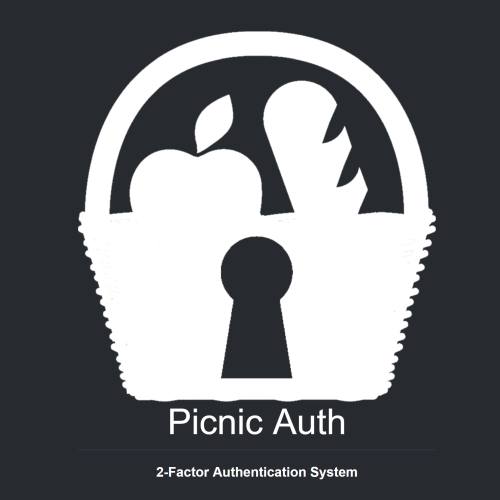
\includegraphics[width=\textwidth]{content/images/logo}
        \caption{Logo projektu.}
        \label{fig:logo}
    \end{subfigure}
    \begin{subfigure}{0.3\textwidth}
        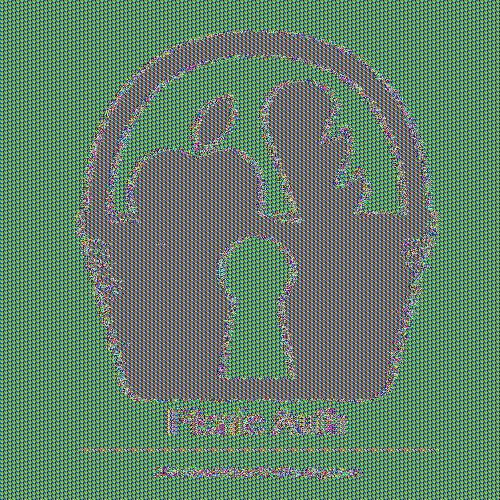
\includegraphics[width=\textwidth]{content/images/logo-ecb}
        \caption{AES w trybie ECB.}
        \label{fig:logo-ecb}
    \end{subfigure}
    \begin{subfigure}{0.3\textwidth}
        
\includegraphics[width=\textwidth]{content/images/logo-cbc}
        \caption{AES w trybie CBC.}
        \label{fig:logo-cbc}
    \end{subfigure}
    \caption{Wizualizacja trybów szyfrowania.}
    \label{modes}
\end{figure} 

\subsubsection{CBC}
Najczęściej używanym trybem jest \textit{CBC - Cipher Block Chaining (ang.)}. 
W tym trybie, blok wiadomości najpierw jest XORowany z poprzednim zaszyfrowanym blokiem a następnie
on sam jest poddawany procesowi szyfrowania. W przypadku pierwszego bloku, dla którego nie ma bloku poprzedniego, 
wprowadzane jest pojęcie \textit{wektora inicjalizującego}. \\ 
Wektor ten powinien być niemożliwy do zgadnięcia a w idealnej sytuacji powinien on być kryptograficznie losowy. Nie jest konieczne, aby wektor inicjalizujący był tajny, zwykle jest wysyłany razem z zaszyfrowaną wiadomością. Ważne jest jednak, aby atakujący nie był w stanie go przewidzieć przed samym procesem szyfrowania. \\ 
Wizualizacja procesu szyfrowania trybem CBC przedstawiona jest na Rysunku \ref{cbc-enc}. \\
Proces deszyfrowania jest analogiczny. W pierwszej kolejności, zaszyfrowany blok poddawany jest działaniu szyfru 
blokowego, po czym jest on XORowany z poprzednim zaszyfrowanym blokiem. Na pierwszy blok musi zostać użyta funkcja XOR
z takim samym wektorem inicjalizującym, jaki został użyty podczas szyfrowania. \\ 
Schemat ten przedstawiony jest na Rysunku \ref{cbc-dec}. \\\\
Tryb CBC sam w sobie można uznać za bezpieczny (w odróżnieniu od ECB), 
należy jednak pamiętać o paru najczęściej popełnianych błędach:
\begin{enumerate}
	\item Używanie tego samego wektora inicjalizującego dla więcej niż jednej wiadomości.
	\item Używanie przewidywalnych wektorów inicjalizujących, na przykład bazujących na liczniku.
	\item Używanie klucza jako wektora inicjalizującego. 
\end{enumerate}
Jednym z najbardziej znanych ataków na system bazujący na trybie CBC był atak o nazwie \textit{BEAST} \cite{beast}. 
Błędem, który został wykorzystany, było użycie zaszyfrowanego bloku poprzedniej wysłanej wiadomości jako wektora inicjalizującego. \\
Porównanie skuteczności tego trybu z trybem ECB przedstawione jest na Rysunku \ref{modes}.
\begin{figure}
    \centering
	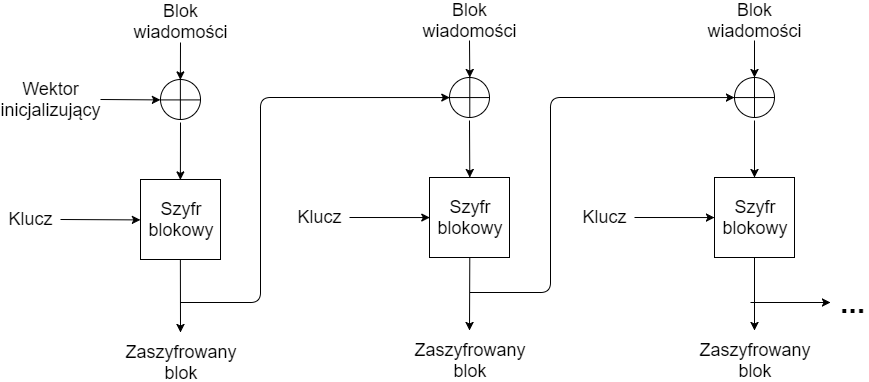
\includegraphics[width=\textwidth]{content/images/cbc-enc-scheme}
    \caption{Schemat szyfrowania w trybie CBC.}
    \label{cbc-enc}
\end{figure}
\begin{figure}
    \centering
	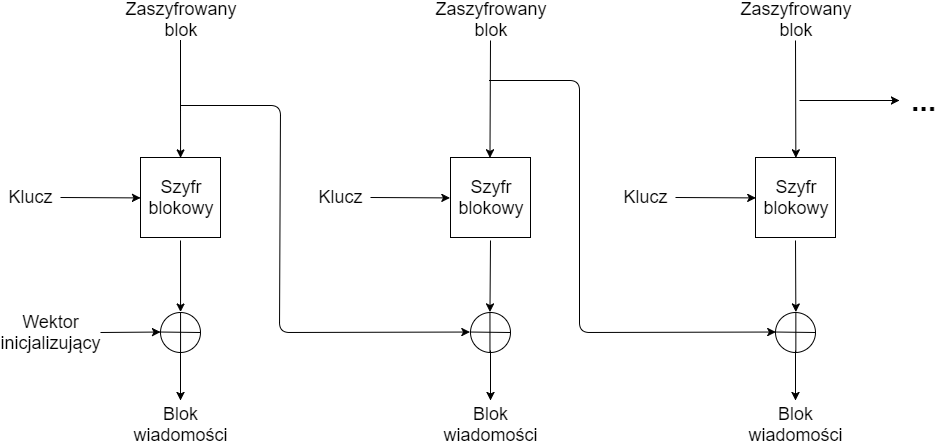
\includegraphics[width=\textwidth]{content/images/cbc-dec-scheme}
    \caption{Schemat deszyfrowania w trybie CBC.}
    \label{cbc-dec}
\end{figure}

\subsubsection{CTR}
Warto wspomnieć jeszcze o trybie \textit{CTR - Counter (ang.)}, gdyż sposób jego działania jest zbliżony 
do szyfrów strumieniowych. Wykorzystywany jest w nim \textit{liczba używana jednorazowo (z angielskiego ,,nonce'')}
oraz licznik. Licznik jest zwiększany dla każdego z bloków wiadomości. 
Na wejście szyfru blokowego podawana jest wyżej wspomniana liczba połączona z licznikiem. Następnie wynik
działania szyfru jest XORowany z blokiem wiadomości. \\
Krytyczne jest tutaj generowanie nowej liczby \textit{nonce} dla każdej z wiadomości. \\
Wizualizacja tego trybu szyfrowania przedstawiona jest na Rysunku \ref{ctr-enc} oraz na Rysunku \ref{ctr-dec}.

\begin{figure}[t]
    \centering
	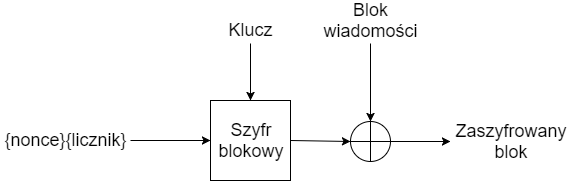
\includegraphics[width=\textwidth]{content/images/ctr-enc-scheme}
    \caption{Schemat szyfrowania w trybie CTR.}
    \label{ctr-enc}
\end{figure}
\begin{figure}[t]
    \centering
	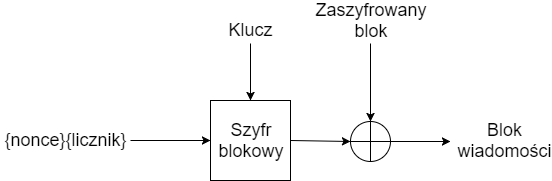
\includegraphics[width=\textwidth]{content/images/ctr-dec-scheme}
    \caption{Schemat deszyfrowania w trybie CTR.}
    \label{ctr-dec}
\end{figure}

\subsection{Data Encryption Standard}
Szyfr blokowy DES był pierwszym algorytmem, zatwierdzonym przez \textit{Narodowe Biuro Standaryzacji} 
(obecnie \textit{Narodowy Instytut Standaryzacji i Technologii}), jako bezpieczny standard szyfrowania symetrycznego.
Przez ponad 20 lat stowarzyszenia naukowe poddawały go intensywnym analizom. \\
W tym czasie został wielokrotnie złamany, głównie z powodu długość klucza jaką posiada szyfr - zaledwie 56 bitów. \\
Jednym ze skutecznych ataków na DES było przedsięwzięcie, dokonane w styczniu 1999 roku, składające się z kooperacji platformy \textit{distributed.net} 
oraz urządzenia stworzonego przez \textit{Electronic Frontier Foundation} o nazwie \textit{Deep Crack}. 
Atak bazował wyłącznie na metodzie siłowej, należało więc sprawdzić $2^{56} = 72\ 057\ 594\ 037\ 927\ 936$ różnych kluczy.
W mniej niż 24 godziny szyfr DES został sukcesywnie złamany. \\
Dla porównania przy dzisiejszej mocy obliczeniowej może on zostać złamany przez jedną maszynę w około jeden dzień \cite{desday}. \\
Próbą uratowania szyfru była propozycja algorytmu 3DES. 
Polegał on na zaszyfrowaniu danych szyfrem DES, odszyfrowaniu ich, a następnie ponownym zaszyfrowaniu. 
Zamiast 3-krotnego szyfrowania, 3DES został wybrany schemat operacji umożliwiający zachowanie kompatybilności z systemami, w których możliwe było użycie jedynie wersji podstawowej algorytmu. \\
Pomimo zwiększonej długości klucza w przypadku 3DES, w porównaniu do AES jest mniej bezpieczny i nadzwyczajnie wolny (AES potrzebuje 12.6 cykli procesora do zaszyfrowania bajtu danych, 3DES aż 134.5 \cite{crypto101}).

\subsection{Advanced Encryption Standard}
Po problemach z DES agencja NIST ogłosiła konkurs na algorytm, który mógłby stać się nowym standardem.
Do konkursu zgłoszone zostały między innymi: \textit{Rijndael}, \textit{Serpent}, \textit{Twofish}, \textit{MARS} czy \textit{RC6}. 
Zostały one poddane intensywnej kryptoanalizie. 
Ostatecznie wygrał algorytm stworzony przez Vincenta Rijmena oraz Joana Daemena - Rijndael. \\
Rijndael jest rodziną szyfrów, których rozmiar bloku oraz rozmiar klucza może wynosić: 128, 160, 192, 224 i 256 bitów. 
Za standard (AES) uznany został Rijndael z długością bloku równą 128 bitów oraz rozmiarze klucza równym 128, 192 lub 256 bitów. \\ \\
Algorytm składa się z wielu przebiegów. Liczba przebiegów zależy od rozmiaru klucza. \\
Pierwszym etapem algorytmu jest rozszerzenie klucza. 
Jako że, w każdym przebiegu potrzebny jest 128-bitowy klucz, zachodzi konieczność wygenerowania wielu kluczy, 
na podstawie głównego klucza. \\
W pierwszej kolejności główny klucz jest ładowany do macierzy 4 na 4 bajty. 
Ostatnia kolumna jest obracana (bajt z góry jest wstawiany na dół) a następnie 
wartość każdej komórki z obróconej kolumny podawana jest do nieliniowej funkcji zamiany, 
specyficznej dla algorytmu AES, zamieniającej podany bajt na inny.
Następnie kolumna ta jest XORowana ze stałą przebiegu (inną dla każdego przebiegu). 
Na koniec XORowana jest ona z pierwszą kolumną klucza poprzedniego przebiegu. \\
Pozostałe kolumny liczone są XORując poprzednią kolumnę z kolumną na tym samym miejscu, ale z klucza poprzedniego przebiegu. \\ 
Po wygenerowaniu klucz, algorytm rozpoczyna przebiegi. \\
Każdy przebieg składa się z następujących kroków:
\begin{enumerate}
	\item Zamiana bajtów. \\
			Funkcja zamiany algorytmu AES jest złożeniem dwóch funkcji: $f(g(a_{xy})).$ \\
			Wynikiem wewnętrznej funkcji \textit{g} jest liczba odwrotna do zadanej nad ciałem skończonym.
			Jest to równoznaczne z zamianą zadanej liczby do postaci wielomianowej (wielomian o maksymalnym 
			stopniu równym 7, w którym współczynnikami są bity liczby) a następnie znalezienie takiego
			wielomianu, który po przemnożeniu przez wielomian liczby, modulo $x^8+x^4+x^3+x+1$, da w wyniku 1. \\
			Funkcja \textit{f} jest przedstawiona na Rysunku \ref{ff}.  \\
			\begin{figure}[t]
			    \centering
			    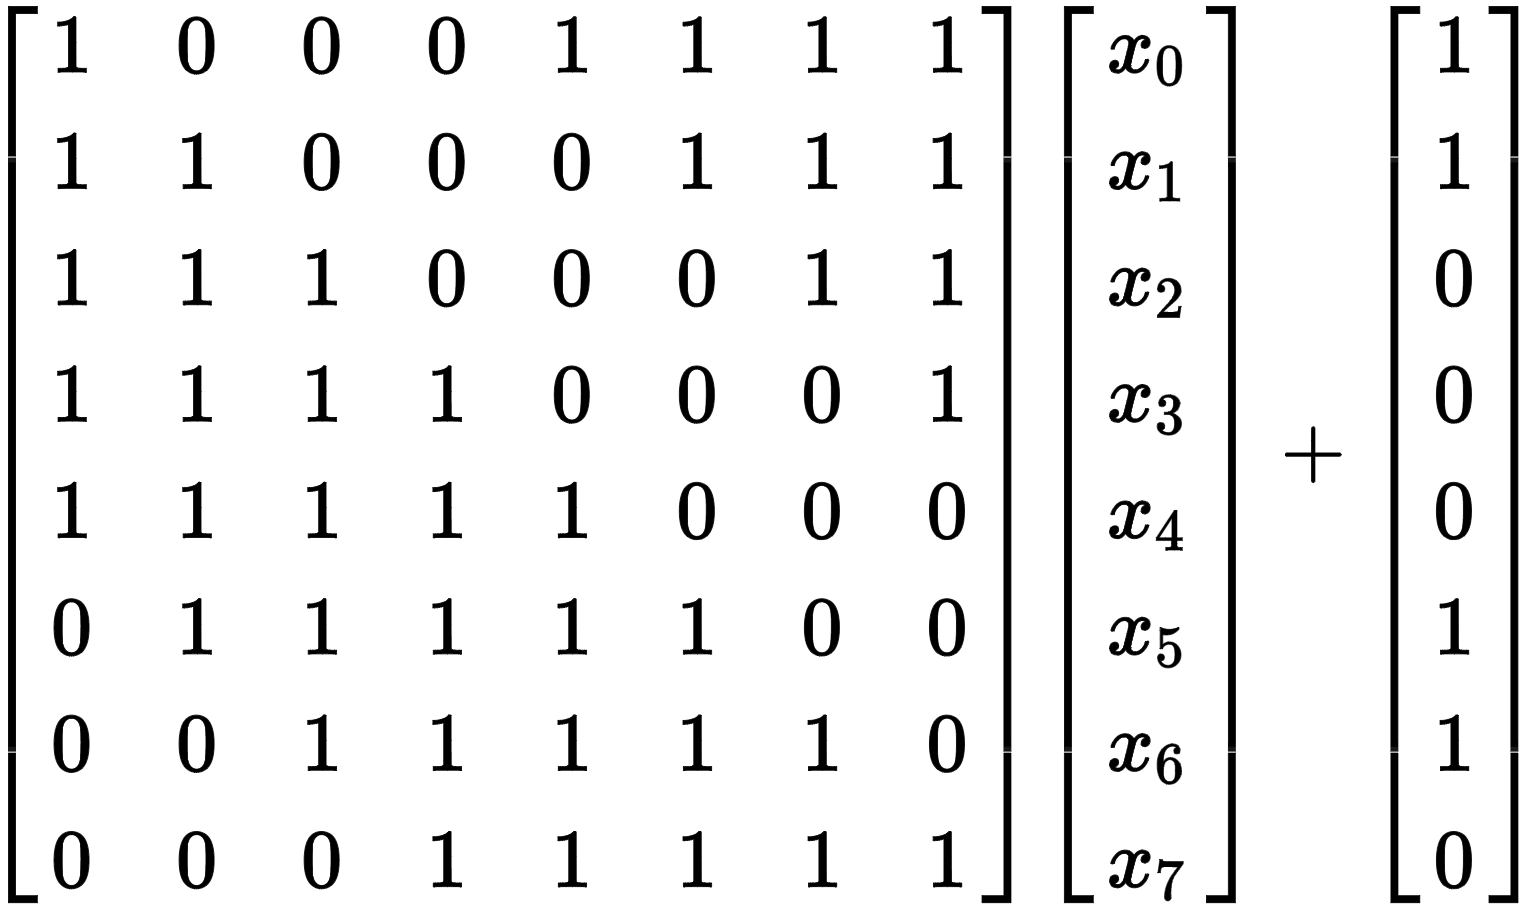
\includegraphics[scale=0.5]{content/images/affin}
				\caption{Przekształcenie \textit{f}.}
				\label{ff}
			\end{figure}
			Możliwe jest też jednorazowe wygenerowania tablicy odwzorowania (przedstawiona na Rysunku \ref{matrix}) dla zadanych wielomianów,
			dzięki czemu zamiast za każdym razem obliczać wartość tej funkcji, wystarczy odczytać wartość tablicy
			pod odpowiednim indeksem. 
			\begin{figure}[t]
			    \centering
			    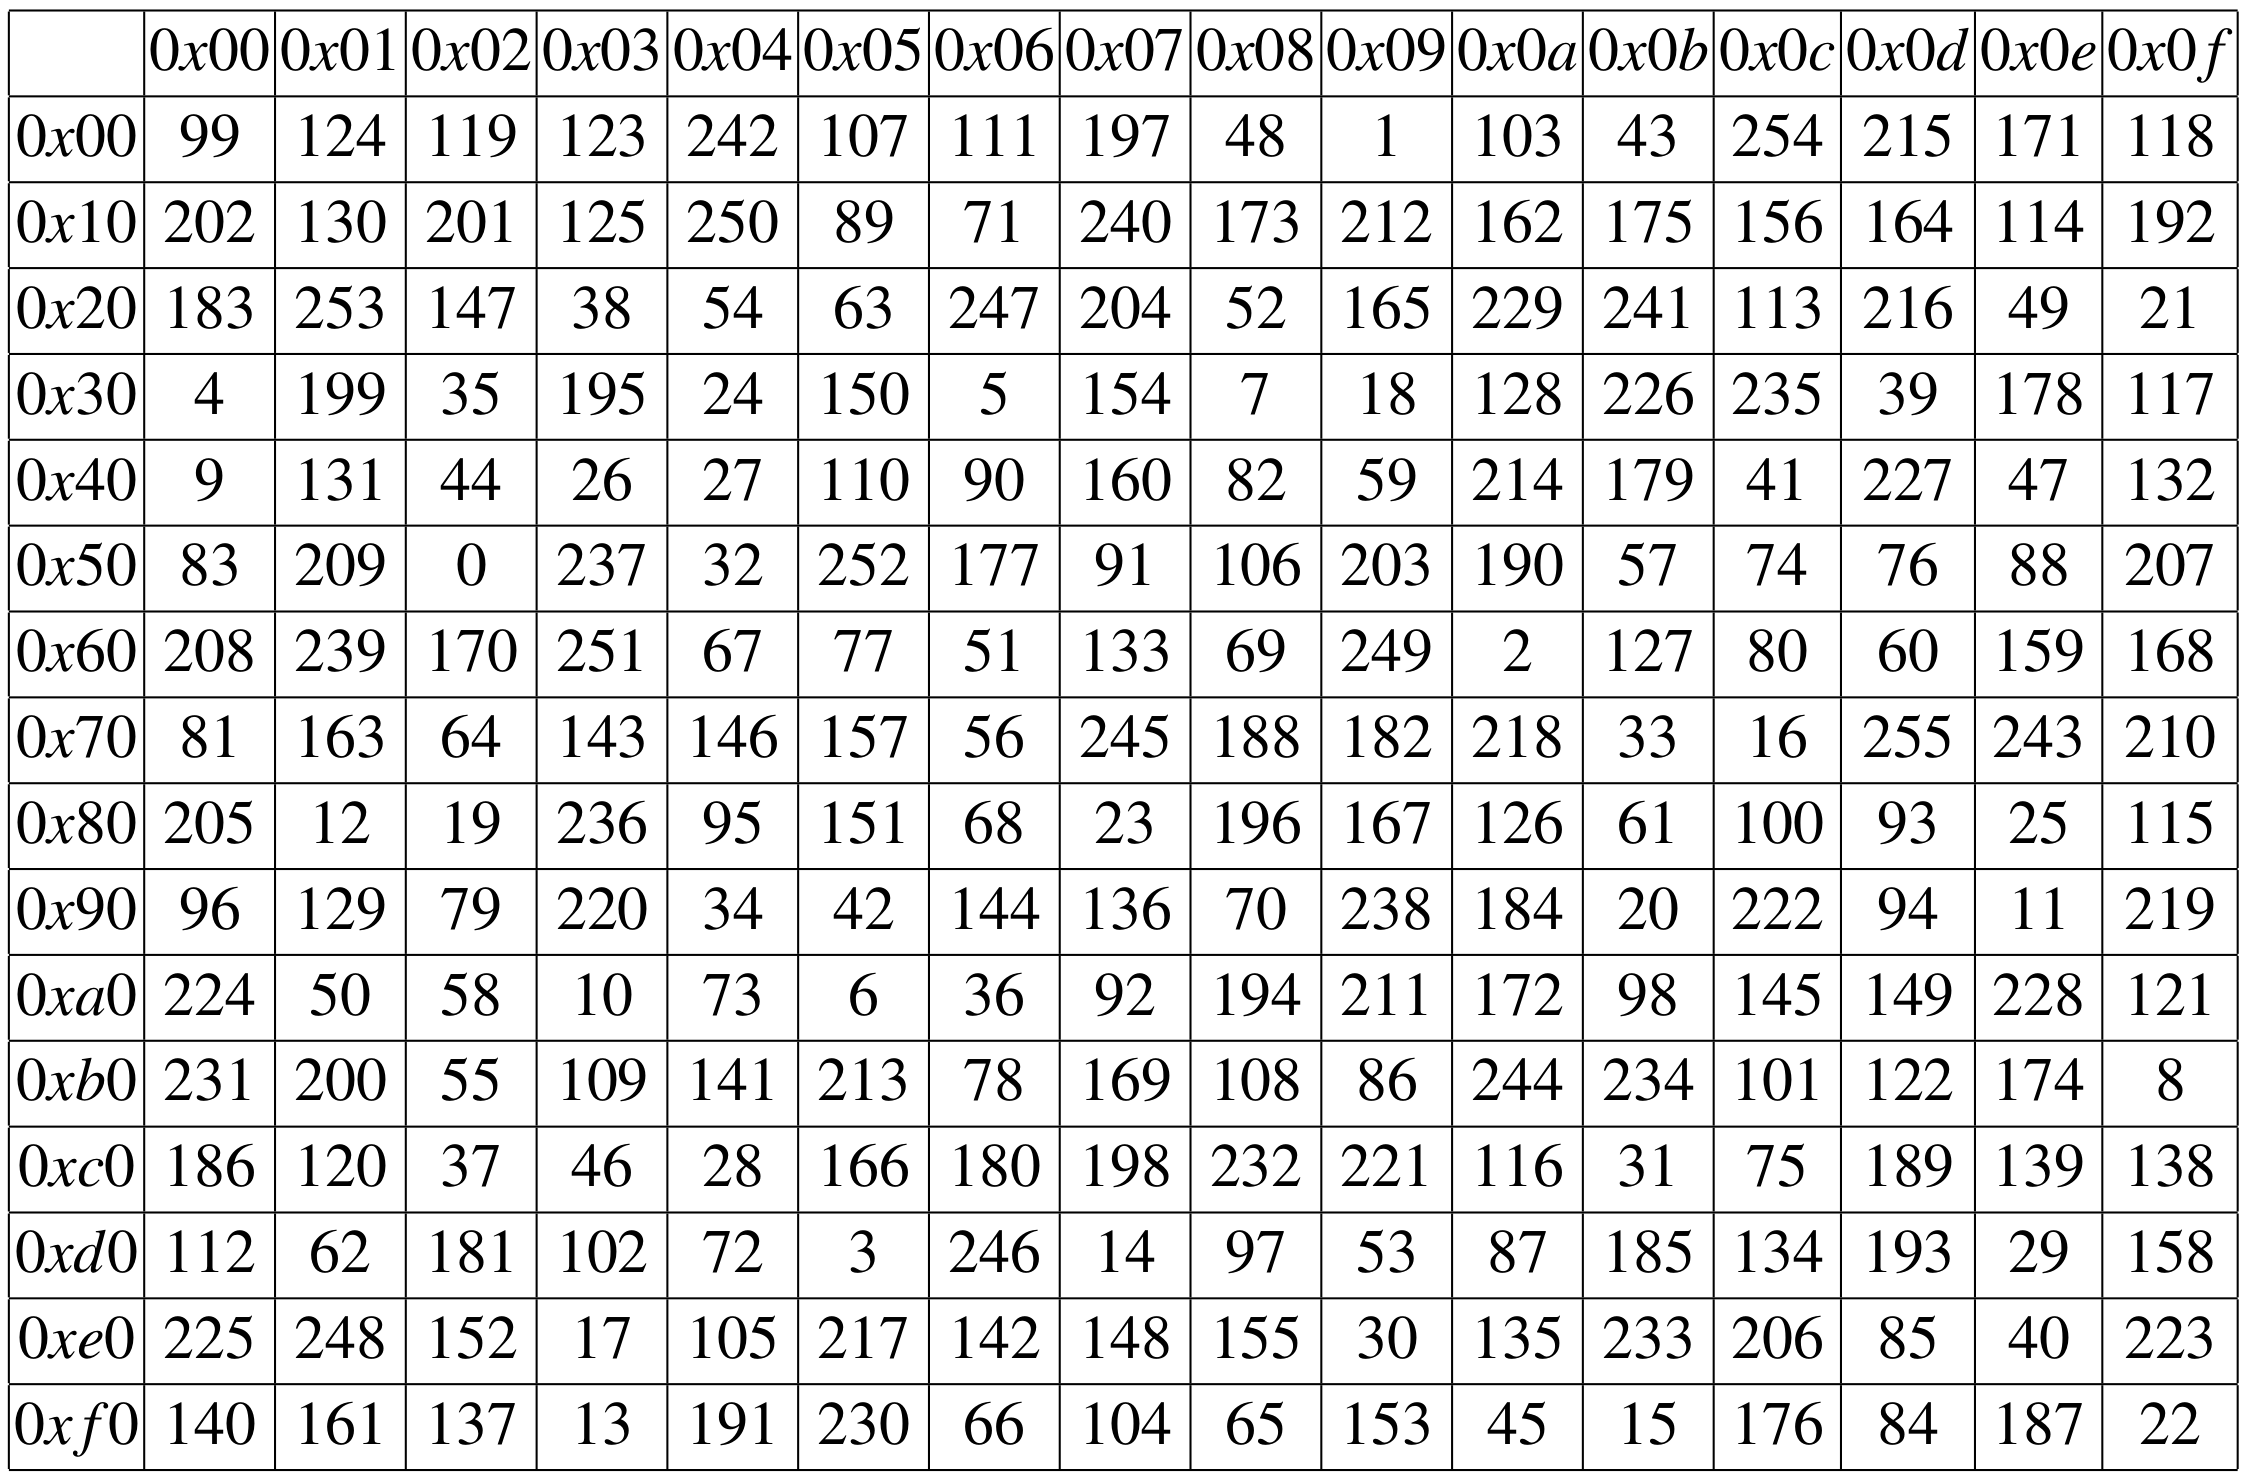
\includegraphics[width=\textwidth]{content/images/sbox}
				\caption{Macierz odwzorowania funkcji zamiany.}
				\label{matrix}
			\end{figure}
			Przykładowo bajt 0xc4, za pomocą powyższej tablicy, konwertowany jest do wartości~28.
			\begin{figure}[t]
			    \centering
			    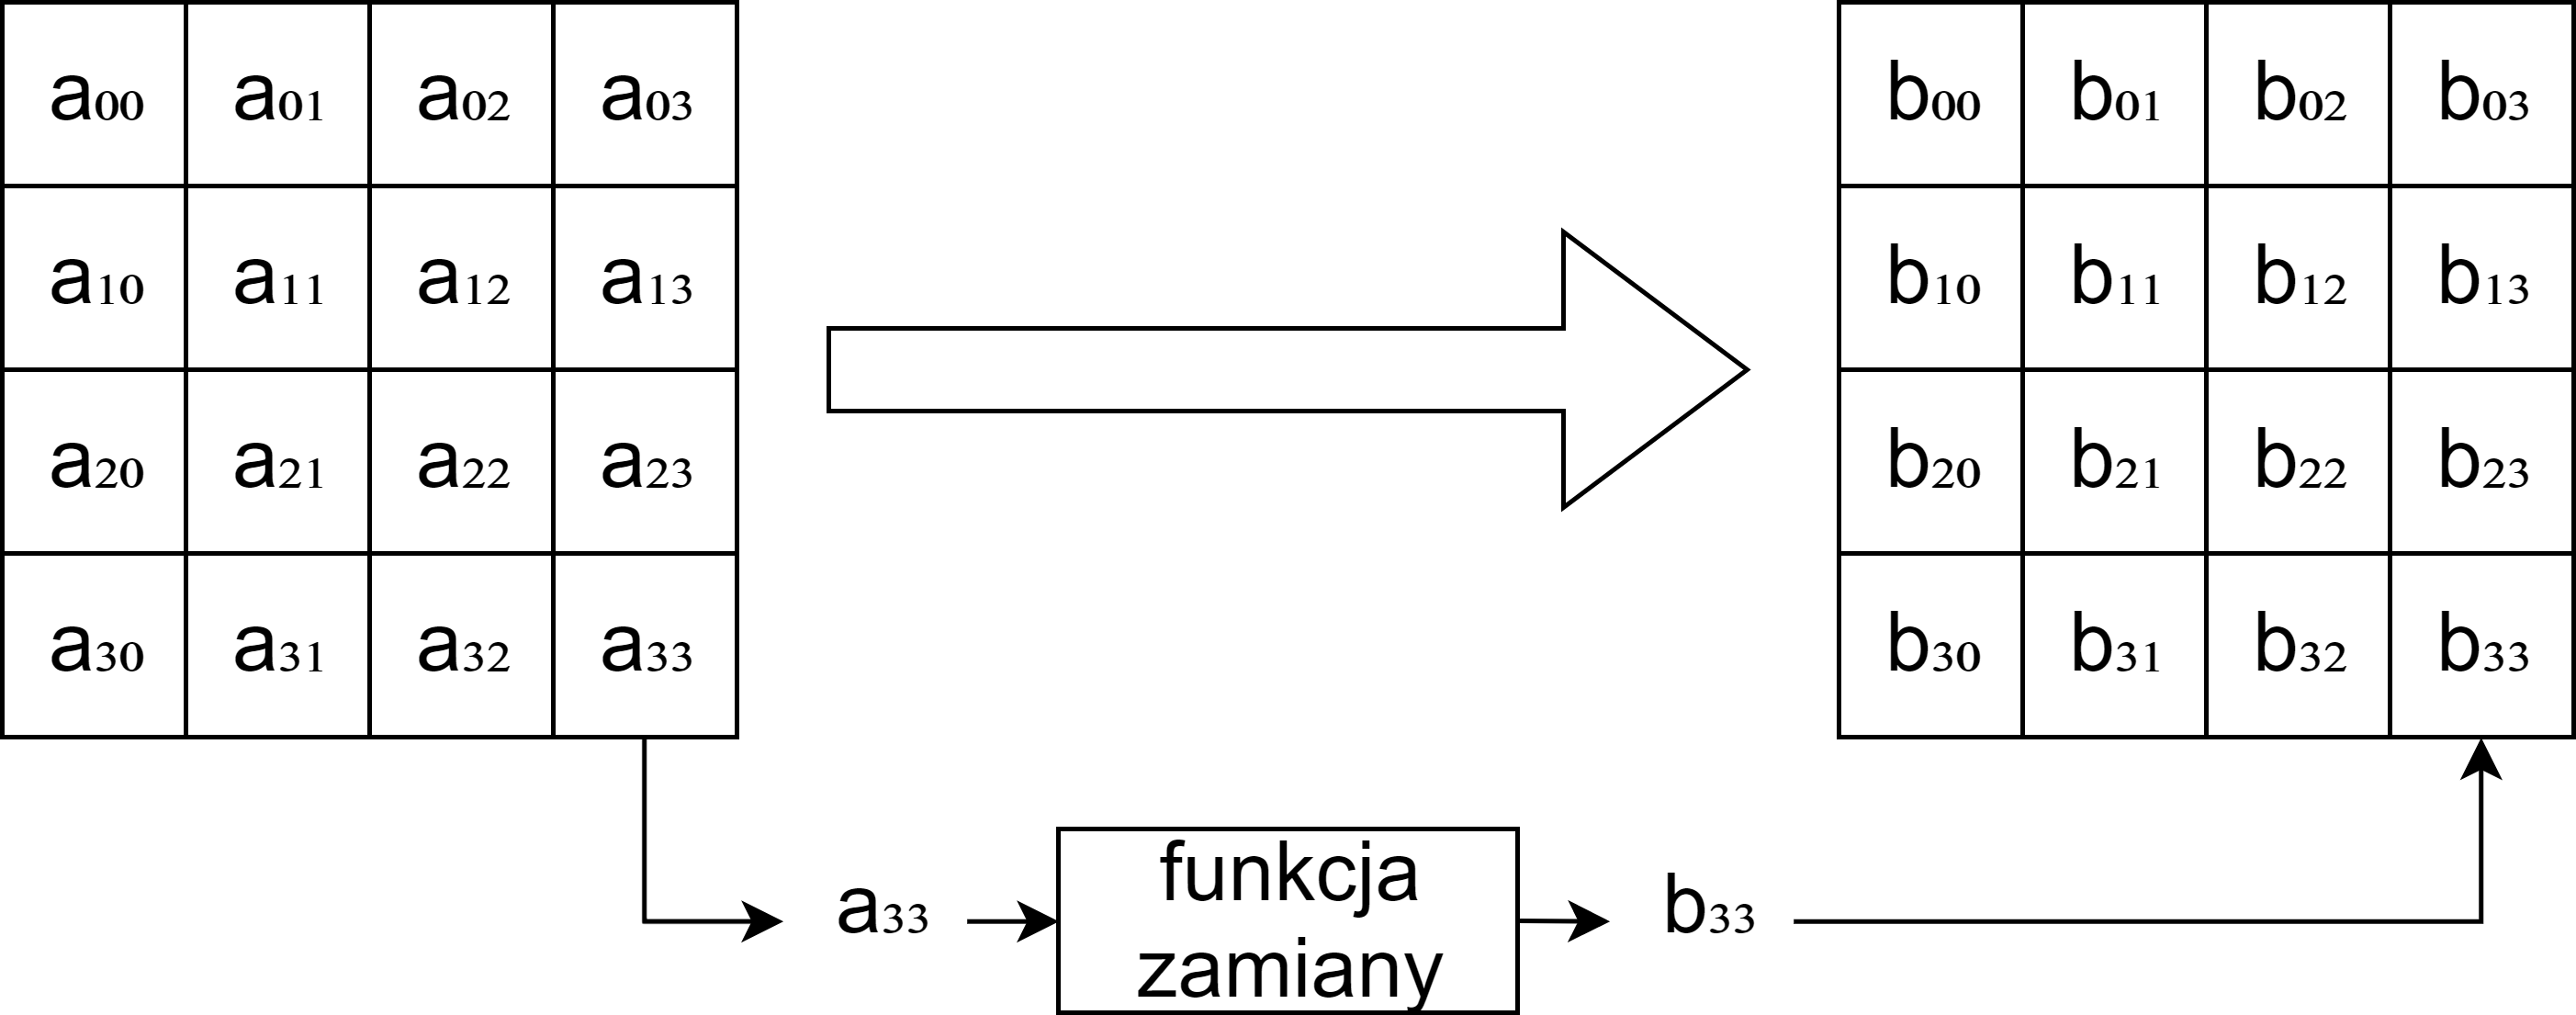
\includegraphics[width=\textwidth]{content/images/sub-bytes}
				\caption{Wizualizacja zamiany bajtów.}
				\label{change}
			\end{figure}
			Wizualizacja zamiany bajtów przedstawiona jest na Rysunku \ref{change}.
	\item Przesuwanie wierszy. \\
			Każdy z wierszy jest przesuwany o odpowiednio 0, 1, 2, 3 komórki w lewo. 
			Komórki macierzy, które wyszły poza macierz są dostawiane z prawej strony.
			\begin{figure}[t]
			    \centering
			    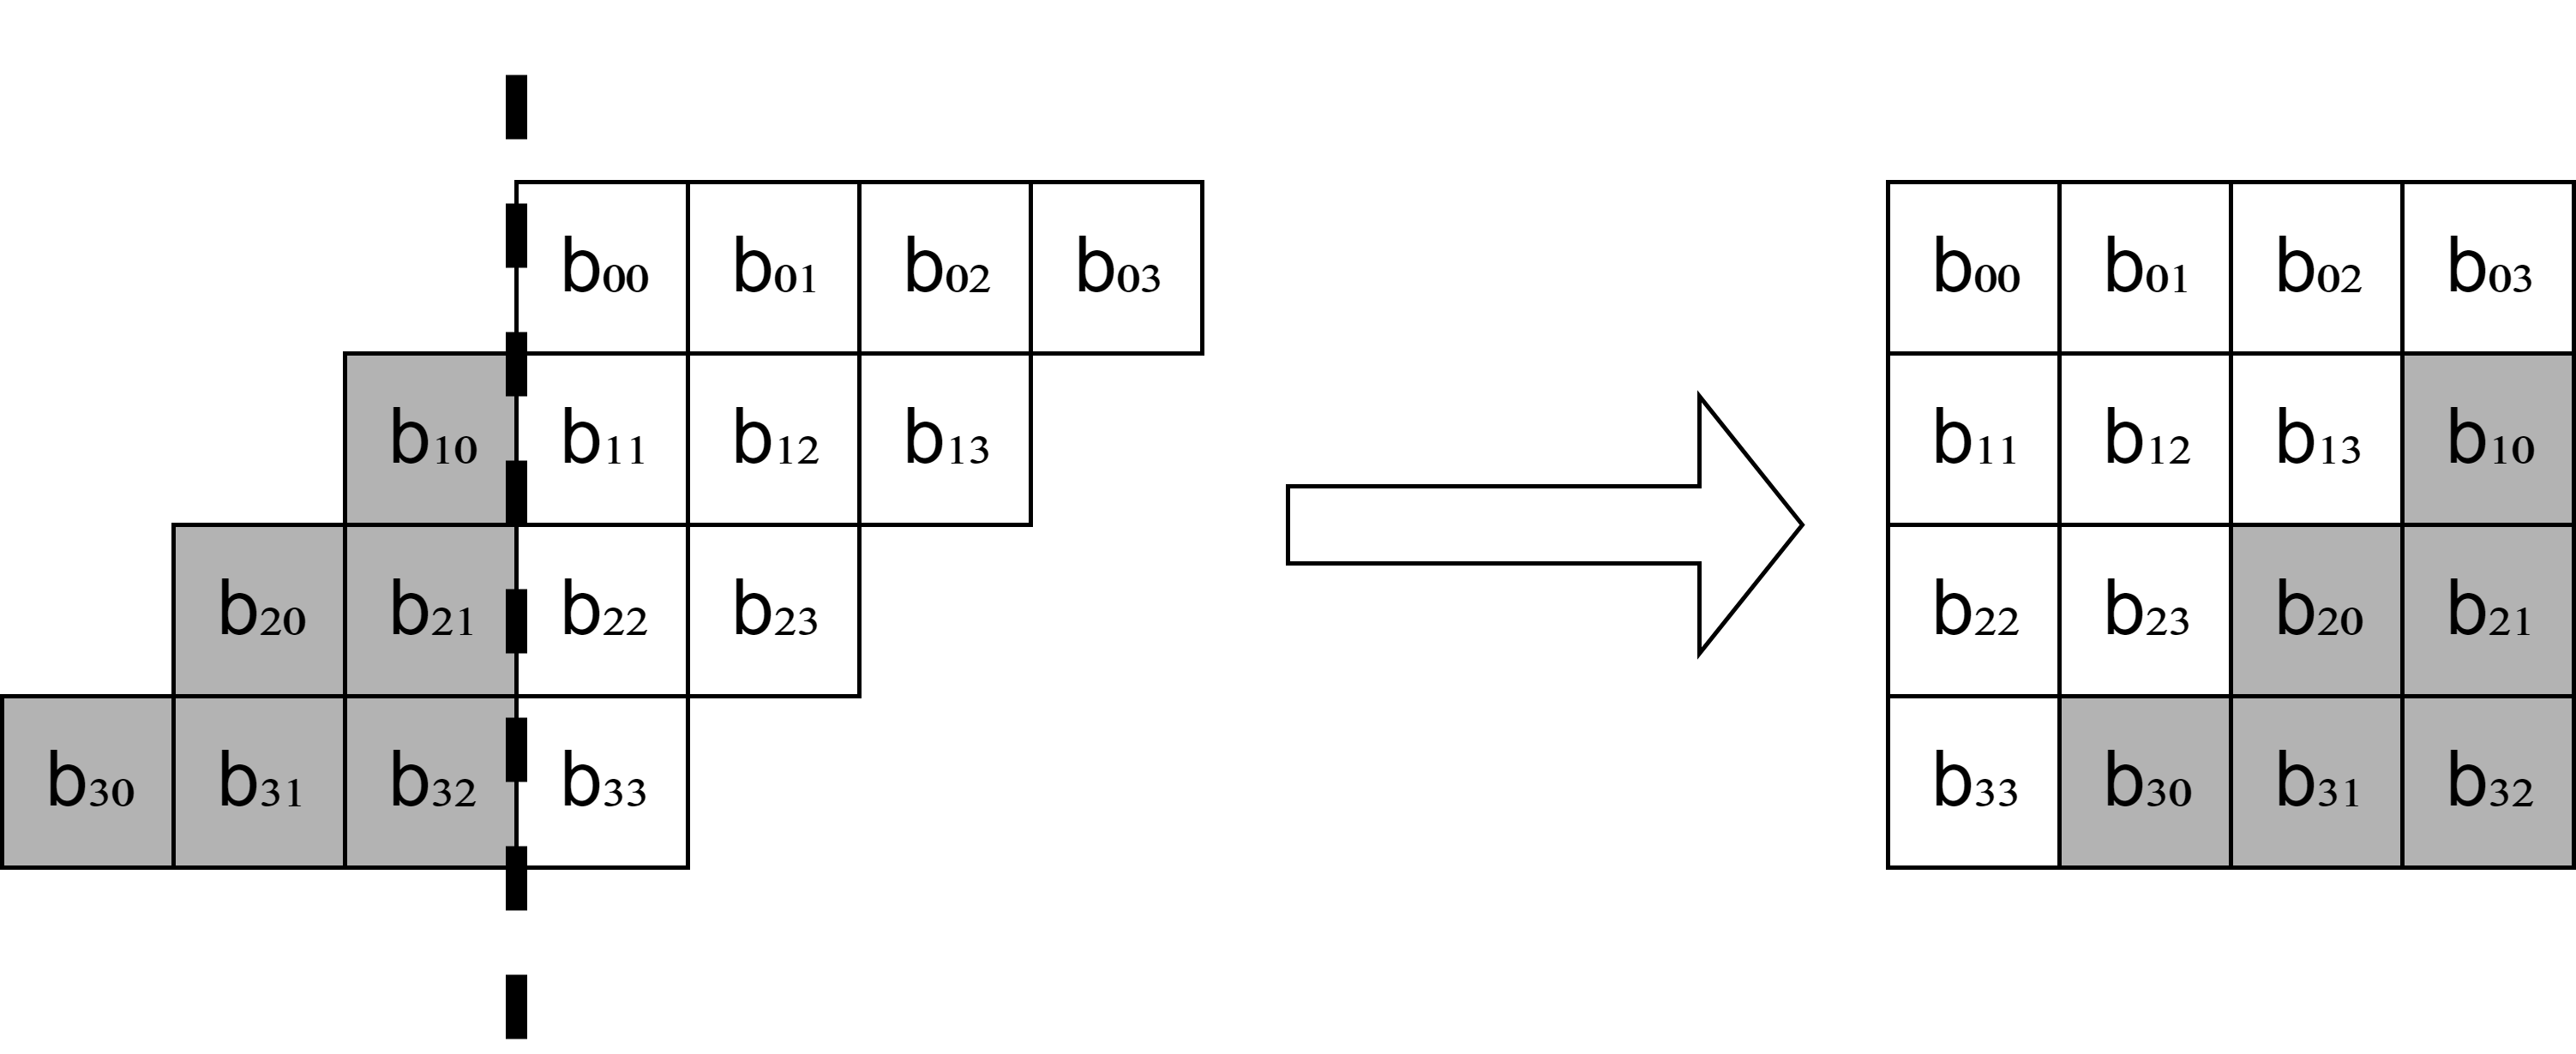
\includegraphics[width=\textwidth]{content/images/shift-row}
				\caption{Wizualizacja przesunięcia wierszy.}
				\label{rows}
			\end{figure}
			Wizualizacja przesuwania wierszy przedstawiona jest na Rysunku \ref{rows}.
	\item Mieszanie kolumn. \\
			Kolumna zapisywana jest w postaci wielomianu, następnie 
			wielomian ten jest mnożony przez specjalny wielomian $03x^3+01x^2+01x+02$. 
			Na koniec brana jest reszta z dzielenia przez wielomian $x^4 + 1$. \\ 
			Całość powyższych operacji można uprościć do mnożenia macierzowego: 
			$$
				\begin{bmatrix}
					2 1 1 3 \\
					3 2 1 1 \\
					1 3 2 1 \\
					1 1 3 2
				\end{bmatrix}
				\times
				\begin{bmatrix}
					b_{01} \\
					b_{12} \\
					b_{23} \\
					b_{30} \\
				\end{bmatrix}
				=
				\begin{bmatrix}
					c_{01} \\
					c_{11} \\
					c_{21} \\
					c_{31} \\
				\end{bmatrix}
			$$
			W przypadku ostatniego przebiegu krok ten jest pomijany.
			\begin{figure}[t]
			    \centering
			    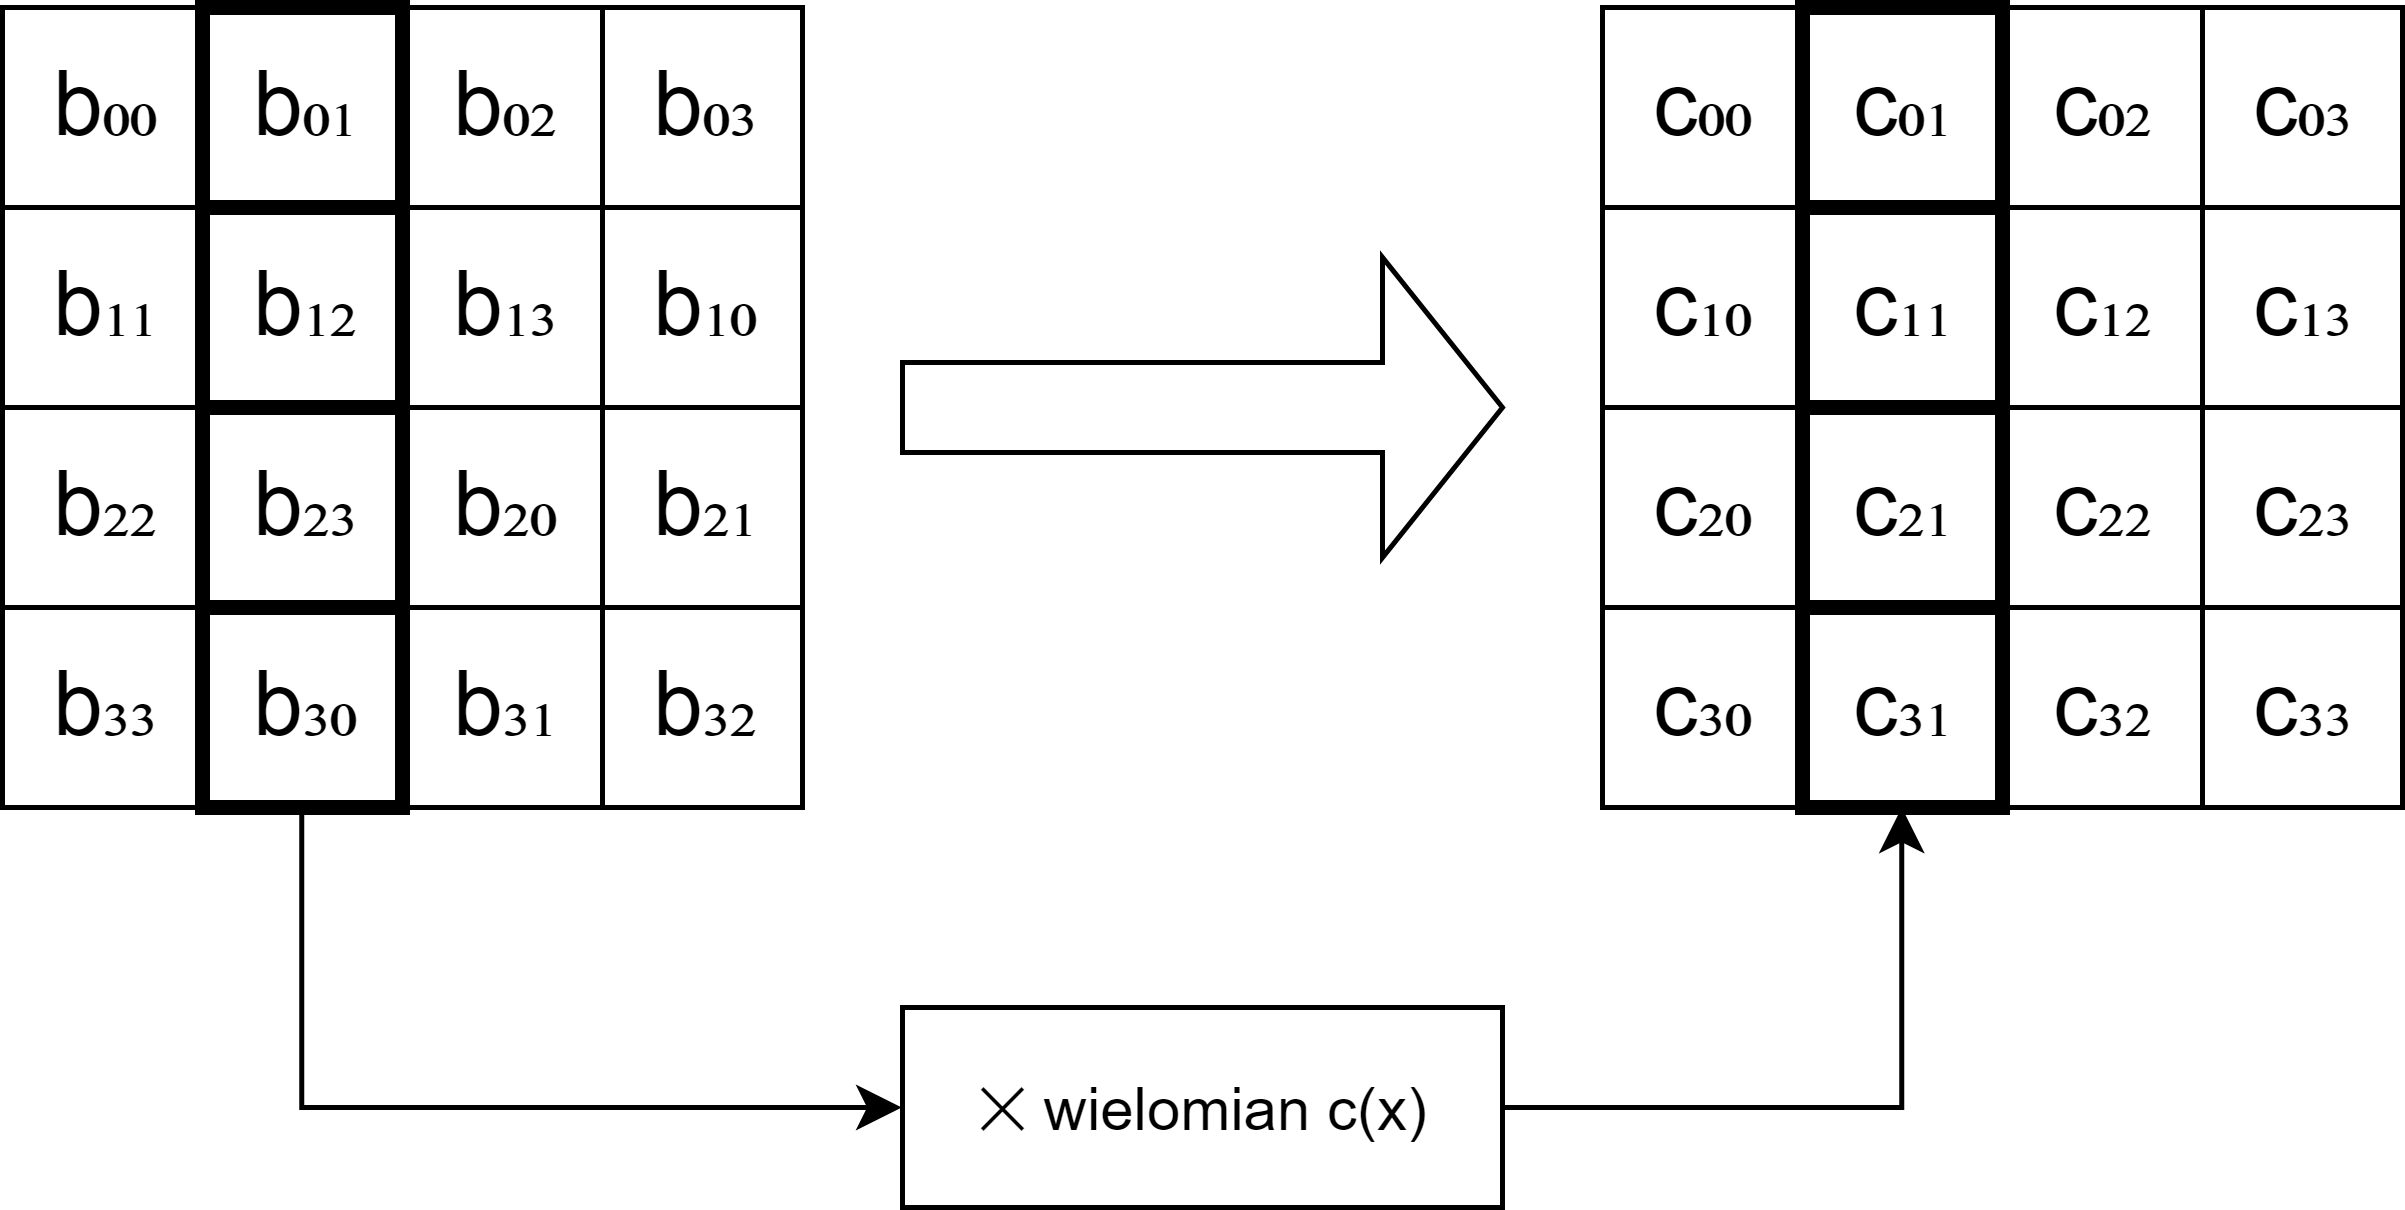
\includegraphics[width=\textwidth]{content/images/mix-cols}
				\caption{Wizualizacja mieszania kolumn.}
				\label{cols}
			\end{figure}
			Wizualizacja mieszania kolumn przedstawiona jest na Rysunku \ref{cols}.
	\item Dodanie klucza przebiegu. \\
			Ostatnim etapem przebiegu jest użycie funkcji XOR pomiędzy każdym elementem macierzy
			a każdym elementem klucza przebiegu.
			\begin{figure}[t]
			    \centering
			    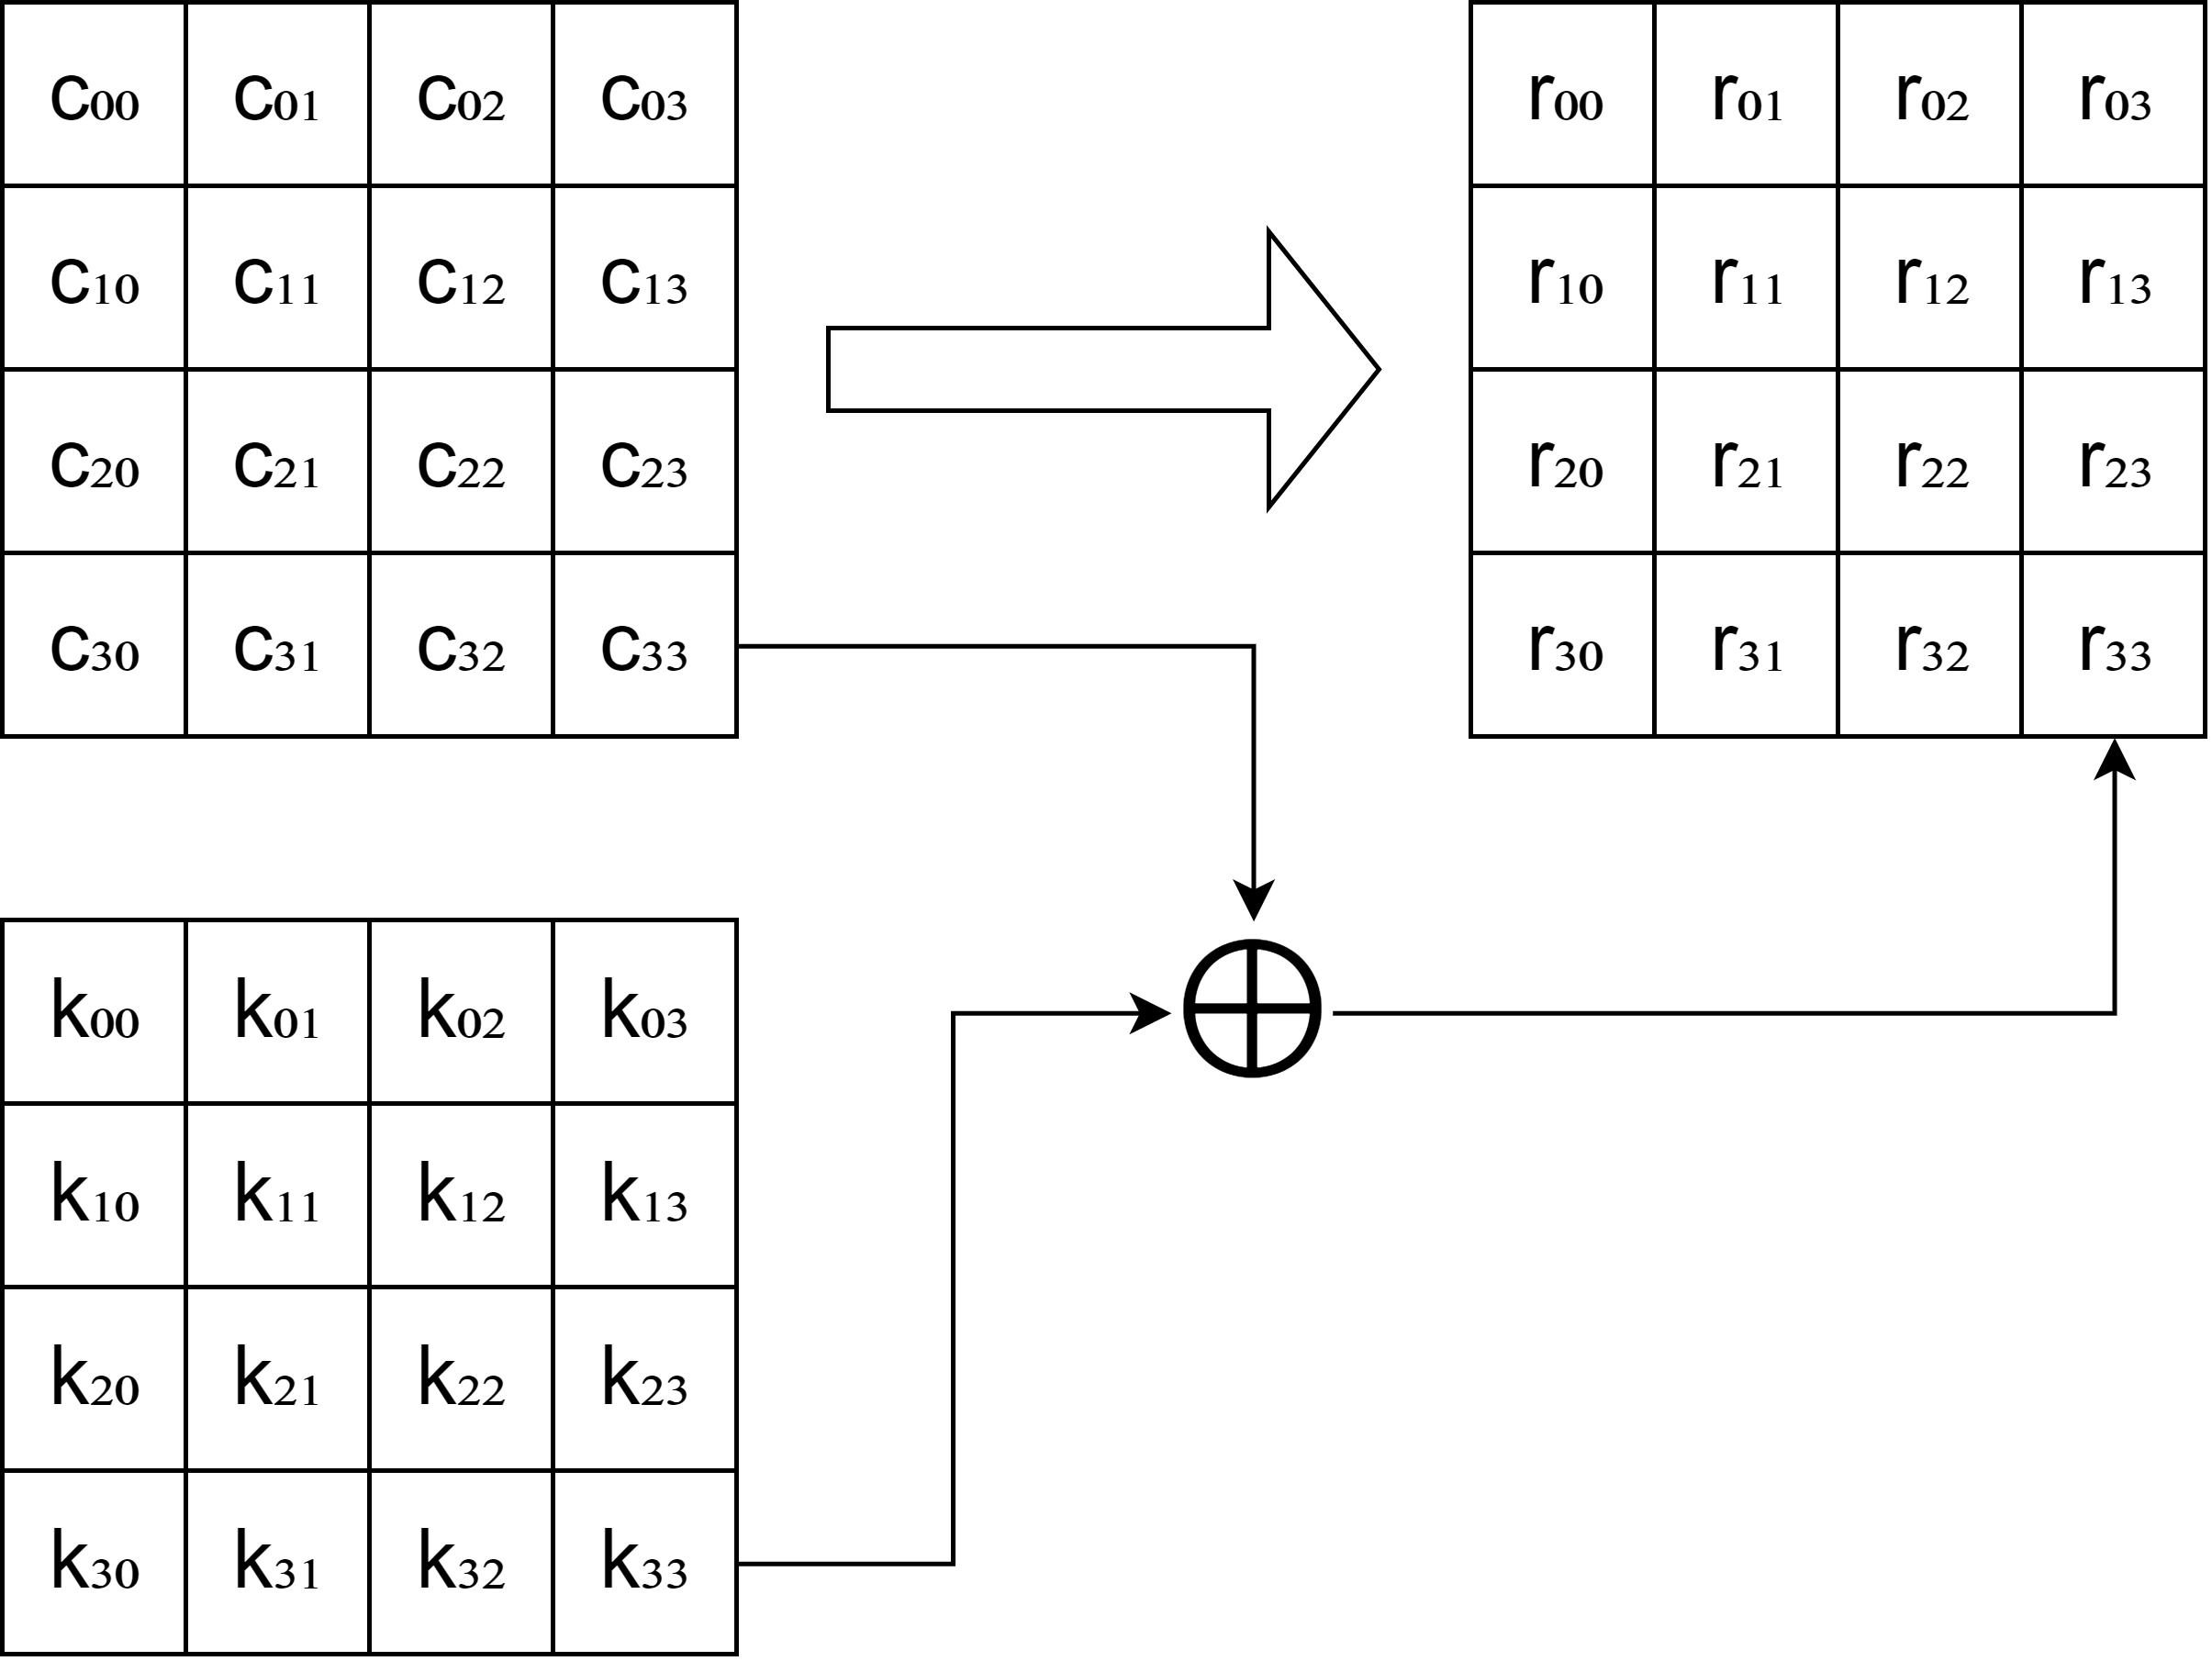
\includegraphics[width=\textwidth]{content/images/add-key}
				\caption{Wizualizacja dodania klucza przebiegu.}
				\label{kk}
			\end{figure}
			Wizualizacja dodania klucza przebiegu przedstawiona jest na Rysunku \ref{kk}
\end{enumerate}
W celu odszyfrowania danych cały proces jest powtarzany w odwrotnej kolejności. \\
Na chwile obecną nie są znane żadne praktyczne ataki na AES a co do szybkości działania na współczesnych komputerach,
znacząco przyczynił się producent procesorów, implementując w nich natywne instrukcje procesora, których 
jedynym zadaniem jest realizacja algorytmu AES.

\section{Szyfry strumieniowe}
Pisząc o szyfrach strumieniowych mam tutaj na myśli natywne szyfry strumieniowe, które zostały stworzone z myślą o pracy w trybie strumieniowym. 
Pomimo istnienia dwóch typów szyfrów strumieniowych - synchroniczny oraz asynchronicznych, w praktyce używany jest prawie wyłącznie pierwszy typ. \\
W odróżnieniu od szyfrów blokowych, które szyfrowały cały blok danych, szyfry strumieniowe szyfrują każdy bit osobno. 
Przy użyciu klucza kryptograficznego generują one wystarczająco długi, pseudolosowy ciąg bitów. 
Następnie wykonywana jest operacja XOR pomiędzy wygenerowanym ciągiem a wiadomością jaką chcemy zaszyfrować. 
Deszyfrowanie polega na ponownym wygenerowaniu ciągu bitów na podstawie klucza a następnie wykonanie operacji XOR na bitach zaszyfrowanej wiadomości oraz tych wygenerowanych z klucza.

\subsection{RC4}
Obecnie najczęściej spotykanym szyfrem strumieniowym jest RC4. Mimo, że wielokrotnie wykazano wiele podatności w konstrukcji RC4, szyfr ten jest ciągle używany w protokołach takich jak TLS czy WEP. \\
Schemat działania algorytmu jest niezwykle prosty. 
Składa się z inicjalizacji klucza oraz generacji pseudolosowego ciągu. \\
W etapie inicjalizacji klucza tworzona jest tablica permutacji S, składają się z 256 bajtów. 
Początkowo znajdują się w niej kolejne liczby od 0 do 255. 
Następnie dokonywane jest przejście po elementach tablicy, korzystając z indeksu \textit{i}. Na każdym kroku pętli obliczany jest indeks \textit{j}, poprzez dodanie aktualnej wartości \textit{j} (zaczynającej się od 0) do wartości klucza znajdującej się pod indeksem \textit{i} oraz do wartości tablicy S znajdującej się pod indeksem \textit{i}. W przypadku, gdyby któryś z indeksu wyszedł poza zakres rozpatrywanych tablic, używa się operacji modulo długość tablicy. Mając obliczony indeks \textit{j} zamienia się element $S[i]$ z elementem $S[j]$. \\
Do wygenerowania pseudolosowego ciągu wykorzystywana jest wcześniej stworzona tablica permutacji S. W pierwszej kolejności dla każdego indeksu \textit{i}, obliczany jest indeks $j := j + S[i]$. 
Następnie zamienione są wartości $S[i]$ oraz $S[j]$. W celu otrzymania bajtu, który zostanie wykorzystany do zaszyfrowania wiadomości, pobierana jest wartość $S[S[i] + S[j]]$ z tablicy~S.

\subsection{Salsa20}
W porównaniu do RC4, Salsa20 jest relatywnie nowym szyfrem strumieniowym, stworzonym przez Daniela J. Bernsteina. 
Bazuje on na operacjach \textit{ARX (add–rotate–xor)}, to jest operacjach składających się z dodawania modulo, obrotów bitowych oraz funkcji \textit{XOR}. 
Zaletą stosowania szyfrów \textit{ARX} jest to, że odporne są one na ataki czasowe, 
polegające na mierzeniu czasu, jaki potrzebny jest do przeprowadzenia operacji kryptograficznych i uzyskiwanie informacji na podstawie wyników pomiarów. \\
Niezwykle interesującą cechą szyfru Salsa20 jest możliwość rozpoczęcia procesu odszyfrowywania od dowolnego miejsca w strumieniu danych. Mając więc duży plik, możliwe jest odszyfrowywanie tylko tej jego części, która nas interesuje. \\
Na chwilę obecną nie są znane żadne praktyczne ataki na szyfr Salsa20, może on zostać użyty jako alternatywa do szyfru blokowego AES.

\section{Kryptograficzna funkcja skrótu}
Funkcją skrótu nazywana jest funkcja, która dla danych wejściowych o dowolnym rozmiarze zwraca dane o z góry ustalonej długości. Funkcje skrótu znajdują zastosowanie w takich dziedzinach jak struktury danych (tablice mieszające, filtr Blooma), algorytmy dopasowania wzorca (algorytm Karpa-Rabina) czy też w kryptografii. \\ \\
Aby funkcja skrótu mogła zostać użyta w systemach kryptograficznych musi posiadać szereg parametrów. \\
Jednym z nich jest odporność na kolizje. Kolizją nazywamy przypadek, gdy dla dwóch różnych argumentów funkcja skrótu zwraca ten sam wynik. Nie jest oczywiście możliwe, aby móc całkowicie uniknąć kolizji, gdyż zbiór danych o dowolnym rozmiarze jest mapowany na zbiór skończony, zależy nam jednak aby proces znajdywania kolizji dla określonych danych był uważany za ,,trudny''. (Przez ,,trudny'' należy tutaj rozumieć problem, który nie jest możliwy do rozwiązania w rozsądnej ilości czasu.) \\
Kolejny z parametrów jest częściowo związany z poprzednim. Zależy nam, aby rozpatrywana funkcja była funkcją jednokierunkową. Oznacza to, że dla danego wyniku funkcji skrótu, znalezienie argumentu jest również problemem ,,trudnym''.
(Sam fakt istnienia funkcji jednokierunkowych nie został formalnie udowodniony. \cite{oneway}) \\
Niezwykle ważne jest też, aby nawet niewielka zmiana danych wejściowych, spowodowała znaczną zmianę danych otrzymanych na wyjściu (wymagane jest aby przynajmniej połowa bitów uległa zmianie).

\subsection{Message Digest 5}
Funkcja MD5 jest wykorzystywana do generowania 128-bitowego skrótu. Została stworzona przez Rona Rivesta w 1991 roku. \\
W uproszczeniu, algorytm MD5 można przedstawić w następujących krokach \cite{crypto101}:
\begin{enumerate}
	\item Dodanie dopełnienia. W pierwszej kolejności dopisywany jest jeden bit o wartości 1, a następnie dopisywane są zera, aż do momentu, gdy długość danych wynosić będzie 448 bitów modulo 512. Dopełnienie dopisywane jest nawet w przypadku, gdy długość danych wynosi 448 bitów.
	\item Pozostałe 64 bity wypełniane są liczbą reprezentującą długość wiadomości (sprzed dopełnienia) modulo $2^{64}$. 
	\item Inicjalizacja stanu MD5 w postaci czterech 32-bitowych zmiennych A, B, C i D. Są one inicjalizowane stałymi zdefiniowanymi w specyfikacji algorytmu (przedstawione w systemie szesnastkowym): \\
		$A := 01 23 45 67$ \\
		$B := 89 ab cd ef$ \\
		$C := fe dc ba 98$ \\
		$D := 76 54 32 10$ 
	\item Dane wejściowe dzielone są na bloki po 512 bitów. Kolejno na każdym z bloków wykonywane są operacje bitowe zmieniające stan zmiennych. 
	\item Wynikiem działania algorytmu jest 128-bitowa wartość składająca się z czterech zmiennych w kolejności A, B, C, D.
\end{enumerate} 
Szczegółowa specyfikacja algorytmy znajduje się w dokumencie RFC 1321 \cite{md5rfc}. \\
Analiza kryptograficzna funkcji MD5 wykazała wiele podatności i błędów przez co obecnie nie jest wskazane używanie MD5 w zastosowaniach kryptograficznych. 
W roku 2004 została opublikowana praca wykazująca podatność funkcji MD5 na ataki kolizyjne (ang. collision attack) \cite{md5cert}. 

\subsection{Secure Hash Algorithm 1}
SHA-1 jest funkcją bazującą na MD4 (podobnie jak MD5), o długości skrótu wynoszącej 160 bitów \cite{cryptoirf}. \\
Wewnętrzny stan funkcji składa się z pięciu zmiennych: A, B, C, D oraz E, każda o rozmiarze 32 bitów. \\
Pseudokod algorytmu można przedstawić w następujących krokach:
\begin{enumerate}
	\item Inicjalizacja zmiennych następującymi stałymi: \\
		$A := 1732584193$ \\
		$B := 4023233417$ \\
		$C := 2562383102$ \\
		$D := 271733878$ \\
		$E := 3285377520$ 
	\item Zaaplikowanie dopełnienia:
		\begin{enumerate}
			\item Dopisanie na koniec danych bitu o wartości 1. \\ 
			Przykładowo jeśli przetwarzane są dane \textit{01011001}, to są one dopełniane do \textit{010110011}.
			\item Następnie dopisywane są bity o wartości 0, aż do momentu, gdy długość danych wynosić będzie 448 bitów modulo 512. \\
			Mając dane \textit{00101101 01000010 10011101 10001010 00101101 10011101}, po zastosowaniu dopełnienia z kroku (a) otrzymujemy \textit{00101101 01000010 10011101 10001010 00101101 10011101 1}. Jako że długość danych wynosi 49 bitów, wymagane jest dopisanie 399 zer. Po zastosowaniu dopełnienia otrzymujemy (reprezentacja heksadecymalna): \\
			\textit{2d429d8a 2d9d8000 00000000 00000000 \\ 
					00000000 00000000 00000000 00000000 \\ 
					00000000 00000000 00000000 00000000 \\ 
					00000000 00000000 }
			\item W ostatnim kroku na miejsce ostatnich 64 bitów dopisywana jest długość danych. 
			\textit{2d429d8a 2d9d8000 00000000 00000000 \\ 
					00000000 00000000 00000000 00000000 \\ 
					00000000 00000000 00000000 00000000 \\ 
					00000000 00000000 00000000 00000031 }
		\end{enumerate}
	\item Podzielenie wiadomości na 512-bitowe bloki.
	\item Dla każdego z bloków należy wykonać następujące operacje:
		\begin{enumerate}
			\item Podzielenie bloku na szesnaście 32-bitowych części $w[i], 0 \leq i \leq 15$.
			\item Rozszerzenie 16 części do 80 korzystając ze wzoru: \\
				$w[i] := (w[i-3] \xor w[i-8] \xor w[i-14] \xor w[i-16]) << 1$
			\item Inicjalizacja zmiennych pomocniczych dla danego bloku \\
				$a := A$ \\
				$b := B$ \\
				$c := C$ \\
				$d := D$ \\
				$e := E$ 
			\item Dla każdej z 80 części $w[i]$ należy wykonać:
				\begin{enumerate}
					\item jeżeli $0 \leq i \leq 19$ \\
			        	$f := (b \BitAnd c) \BitOr ((\BitNeg b) \BitAnd d)$ \\
			            $k := 0x5A827999$
					\item jeżeli $20 \leq i \leq 39$ \\
           				$f := b \xor c \xor d$ \\
          				$k := 0x6ED9EBA1$
				    \item jeżeli $40 \leq i \leq 59$ \\
			        	$f := (b \BitAnd c) \BitOr (b \BitAnd d) \BitOr (c \BitAnd d)$ \\
           				$k := 0x8F1BBCDC$
        			\item jeżeli $60 \leq i \leq 79$ \\
			            $f := b \xor c \xor d$
   	        			$k := 0xCA62C1D6$
            		\item następnie \\
           				$t := (a <<< 5) + f + e + k + w[i]$ \\
				        $e := d$ \\
				        $d := c$\\
				        $c := b <<< 30$\\
				        $b := a$ \\
				        $a := t$
				\end{enumerate}
			\item Aktualizacja wewnętrznego stanu funkcji \\
				$A := A + a$ \\
				$B := B + b$ \\
				$C := C + c$ \\
				$D := D + d$ \\
				$E := E + e$
		\end{enumerate}
	\item Zwrócenie wyniku w postaci: \\
		$(A << 128) \BitOr (B << 96) \BitOr (C << 64) \BitOr (D << 32) \BitOr E$
\end{enumerate}
W dokumencie RFC 3174 zostały zawarte szczegóły dotyczące algorytmu, jak również przykładowa implementacja \cite{sha1rfc}. \\ \\
Podobnie jak MD5, funkcja SHA-1 również nie jest uważana za bezpieczną. \\
Do roku 2017 wszystkie przedstawione ataki uznawane były za niepraktyczne z uwagi na zbyt dużą moc obliczeniową, jaka byłaby potrzebna do ich wykonania.
Przykładem może być tutaj atak opublikowany w październiku 2015 roku o nazwie \textit{The SHAppening}. Koszt wynajęcia sprzętu potrzebnego do przeprowadzenia ataku (wygenerowania jednej kolizji) estymowany był na 75 000 - 120 000 dolarów amerykańskich \cite{shap}. \\
Pierwszy praktyczny atak na SHA-1 został ogłoszony w lutym 2017 roku. Zostały wygenerowane dwa pliki w formacie PDF, dla których wynik funkcji skrótu SHA-1 jest taki sam. Wszystkie systemy, w których wykorzystywana jest funkcja SHA-1 są narażone na ten atak, przykładowo umożliwia on fałszowanie podpisów cyfrowych dokumentów, czy też certyfikatów HTTPS. \cite{shatt}

\subsection{Secure Hash Algorithm 2}
SHA-2 jest rodziną funkcji składającą się z:
\begin{itemize}
	\item \mbox{SHA-224}
	\item \mbox{SHA-256}
	\item \mbox{SHA-384}
	\item \mbox{SHA-512}
	\item \mbox{SHA-512/224}
	\item \mbox{SHA-512/256} \\
\end{itemize} 
Funkcje te generują skróty o długościach odpowiednio: 
\begin{itemize}
	\item 224
	\item 256
	\item 384
	\item 512
	\item 224
	\item 256 bitów
\end{itemize} 

\subsubsection{SHA-256}
Jedną z najczęściej używanych funkcji z rodziny SHA-2 jest SHA-256. Proces pozyskiwania skrótu SHA-256 jest następujący:
\begin{enumerate}
	\item Inicjalizacja stanu wewnętrznego funkcji: \\
		$A := 1779033703$ \\
		$B := 3144134277$ \\
		$C := 1013904242$ \\
		$D := 2773480762$ \\
		$E := 1359893119$ \\
		$F := 2600822924$ \\
		$G := 528734635$ \\
		$H := 1541459225$
	\item Inicjalizacja pomocniczych stałych. \\
			$$
			k[0..63] := \\
			\begin{matrix}
				1116352408, & 1899447441, & 3049323471, & 3921009573, \\
				961987163,  & 1508970993, & 2453635748, & 2870763221, \\
				3624381080, & 310598401,  & 607225278,  & 1426881987, \\
				1925078388, & 2162078206, & 2614888103, & 3248222580, \\
				3835390401, & 4022224774, & 264347078,  & 604807628,  \\
				770255983,  & 1249150122, & 1555081692, & 1996064986, \\
				2554220882, & 2821834349, & 2952996808, & 3210313671, \\
				3336571891, & 3584528711, & 113926993,  & 338241895,  \\
				666307205,  & 773529912,  & 1294757372, & 1396182291, \\
				1695183700, & 1986661051, & 2177026350, & 2456956037, \\
				2730485921, & 2820302411, & 3259730800, & 3345764771, \\
				3516065817, & 3600352804, & 4094571909, & 275423344,  \\
				430227734,  & 506948616,  & 659060556,  & 883997877,  \\
				958139571,  & 1322822218, & 1537002063, & 1747873779, \\
				1955562222, & 2024104815, & 2227730452, & 2361852424, \\
				2428436474, & 2756734187, & 3204031479, & 3329325298
			\end{matrix}
			$$
	\item Zaaplikowanie dopełnienia. Proces ten przebiega identycznie jak w przypadku SHA-1.
	\item Podzielenie wiadomości na 512-bitowe bloki.
	\item Dla każdego z bloków należy wykonać następujące operacje:
		\begin{enumerate}
			\item Podzielenie bloku na szesnaście 32-bitowych części $w[i], 0 \leq i \leq 15$.
			\item Rozszerzenie 16 części do 64 korzystając ze wzoru: \\
				$s0 := (w[i-15] >>> 7) \xor (w[i-15] >>> 18) \xor (w[i-15] >> 3)$ \\
			    $s1 := (w[i-2] >>> 17) \xor (w[i-2] >>> 19) \xor (w[i-2] >> 10)$ \\
				$w[i] := w[i-16] + s0 + w[i-7] + s1$
			\item Inicjalizacja zmiennych pomocniczych dla danego bloku \\
				$a := A$ \\
				$b := B$ \\
				$c := C$ \\
				$d := D$ \\
				$e := E$ \\
				$f := F$ \\
				$g := G$ \\
				$h := H$
			\item Dla każdej z 64 części $w[i]$ należy wykonać: \\
				$S1 := (e >>> 6) \xor (e >>> 11) \xor (e >>> 25)$ \\
		        $ch := (e \BitAnd f) \xor ((\BitNeg e) \BitAnd g)$ \\
		        $t1 := h + S1 + ch + k[i] + w[i]$ \\
		        $S0 := (a >>> 2) \xor (a >>> 13) \xor (a >>> 22)$ \\
		        $m := (a \BitAnd b) \xor (a \BitAnd c) \xor (b \BitAnd c)$ \\
		        $t2 := S0 + m$ \\
		        $h := g$ \\
		        $g := f$ \\
		        $f := e$ \\
		        $e := d + t1$ \\
		        $d := c$ \\
		        $c := b$ \\
		        $b := a$ \\
		        $a := t1 + t2$
			\item Aktualizacja wewnętrznego stanu funkcji \\
				$A := A + a$ \\
				$B := B + b$ \\
				$C := C + c$ \\
				$D := D + d$ \\
				$E := E + e$ \\
				$F := F + f$ \\
				$G := G + g$ \\
				$H := H + h$ 
		\end{enumerate}
	\item Zwrócenie wyniku w postaci: \\
		$(A << 224) \BitOr (B << 192) \BitOr (C << 160) \BitOr \\ 
		 (D << 128) \BitOr (E << 96) \BitOr (F << 64) \BitOr (G << 32) \BitOr H$
\end{enumerate}
W porównaniu do SHA-1, funkcje SHA-2 są znacznie odporniejsze na kolizję, dzięki czemu zalecane jest ich używanie w zastosowaniach takich jak podpisy cyfrowe czy uwierzytelnianie wiadomości.

\subsection{Secure Hash Algorithm 3}
Wewnętrzna budowa funkcji z rodziny SHA-3 znacząco się różni w odniesieniu do omawianych wcześniej. 
Poprzednie funkcje oparte były o schemat Merkle–Damgård. 
Funkcje z rodziny SHA-3 oparte są o tak zwaną ,,architekturę gąbki''. 
W obu przypadkach funkcja zawiera wewnętrzny stan. 
Różnica jest jednak w sposobie otrzymywania wyniku na podstawie tego stanu. 
Poprzednio zwrócenie przez funkcję wyniku było równoznaczne ze zwróceniem wewnętrznego stanu funkcji. 
W przypadku SHA-3 tak się nie dzieje. Wewnętrzny stan przepuszczany jest kolejne cykle algorytmu. 
Na wynik funkcji składają się części wewnętrznego stanu, pobierane w kolejnych cyklach. 
Skutkuje to tym, że nigdy nie jest ujawniany cały wewnętrzny stan funkcji. \\
Ulepszona wewnętrzna konstrukcja algorytmu zapobiega atakom typu ,,length extension'', 
na który podatne są funkcje MD5, SHA-1 oraz SHA-2 \cite{keccak}.

\section{Uwierzytelnienie i integralność}

\subsection{Kod uwierzytelnienia wiadomości}
W celu zagwarantowania prywatności kanału komunikacji samo szyfrowanie nie jest wystarczające. 
Potwierdzeniem tej tezy są ataki typu \textit{,,Man in the middle''}, w których atakujący podszywa się 
pod osobę, do której przesyłamy wiadomość. Wysyłając wiadomość jesteśmy przekonani, że wysyłamy ją do docelowej osoby,
gdy tak naprawdę wysyłamy ją do atakującego. Odbiorca również sądzi, że otrzymana wiadomość jest wysłana 
przez spodziewanego nadawcę, mimo że wysłał ją atakujący. Pomimo tego, że atakujący nie jest w stanie przeczytać
przechwyconej wiadomości, gdyż jest zaszyfrowana, to może próbować ją modyfikować. \\
Kody uwierzytelnienia wiadomości (Message Authentication Code ang.) są jedną z metod na uwierzytelnienie i zapewnienie 
integralności danych. Przesyłane są razem z wiadomością w formie niewielkiej porcji danych.
Algorytmy generujące MAC przyjmują klucz kryptograficzny o z góry określonej długości oraz dowolne dane 
o dowolnej długości (podobnie jak w przypadku funkcji skrótu) i w wyniku zwracają kod o ustalonej długości.
Algorytmy te umożliwiają również weryfikację danego kodu na podstawie klucza oraz wiadomości. \\
Po wygenerowaniu kodu uwierzytelniającego pozostaje jeszcze kwestia sposobu dołączenia go do wiadomości.
Sposobów tych je wiele. \\
Przykładowo możemy w pierwszej kolejności wygenerować MAC z danej wiadomości a następnie ją zaszyfrować. 
Wysyłana jest wtedy zaszyfrowana wiadomość oraz wygenerowany kod. Jednym z protokołów, w których 
MAC jest wykorzystywany w taki sposób jest protokół SSH. \\
Możliwe jest też wygenerowanie MAC, doklejenie go do wiadomości i zaszyfrowanie całości.
Ten schemat wykorzystywany jest w protokole TLS. \\
Trzecim sposobem jest zaszyfrowanie wiadomości, po czym wygenerowanie MAC z zaszyfrowanej wiadomości.
Tego sposobu używa na przykład protokół IPSec. \\
Okazuje się, że ostatni wspomniany sposób jest najbezpieczniejszy, należy sprawdzić kod uwierzytelnienia wiadomości
przed próbą jej odszyfrowania. W przypadku protokołu SSH, który wykorzystuje pierwszy sposób, istnieje atak, 
który umożliwia atakującemu odszyfrowanie pierwszych czterech bajtów zaszyfrowanego bloku. Jest to spowodowane 
specyficzną konstrukcją pakietu SSH (pole reprezentujące długość pakietu jest również zaszyfrowane).
Na drugi sposób również istnieje atak zaproponowany przez Serge'a Vaudenaya \cite{tls}.

\subsection{MAC bazujący na funkcji skrótu}
Praktycznie jedynym poprawnie działającym mechanizmem generującym kody uwierzytelnienia wiadomości są algorytmy
MAC bazujące na funkcji skrótu (Hash-based Message Authentication Code ang.). 
Oprócz klucza kryptograficznego oraz wiadomości algorytm HMAC pobiera dodatkowo funkcję skrótu. 
Jako argument może zostać użyta dowolna funkcja skrótu: SHA1, SHA-256, SHA-3 czy nawet MD5. 
Nie jest tutaj wymagane aby użyta funkcja skrótu była odporna na kolizję więc HMAC zbudowany na
funkcji MD5 jest uważany za bezpieczny \cite{hmacmd5}, chociaż nie jest to zalecane przy tworzeniu nowych systemów kryptograficznych. \\
Schemat generacji HMAC przedstawia Rysunek \ref{hmac-scheme}.
\begin{figure}[t]
    \centering
	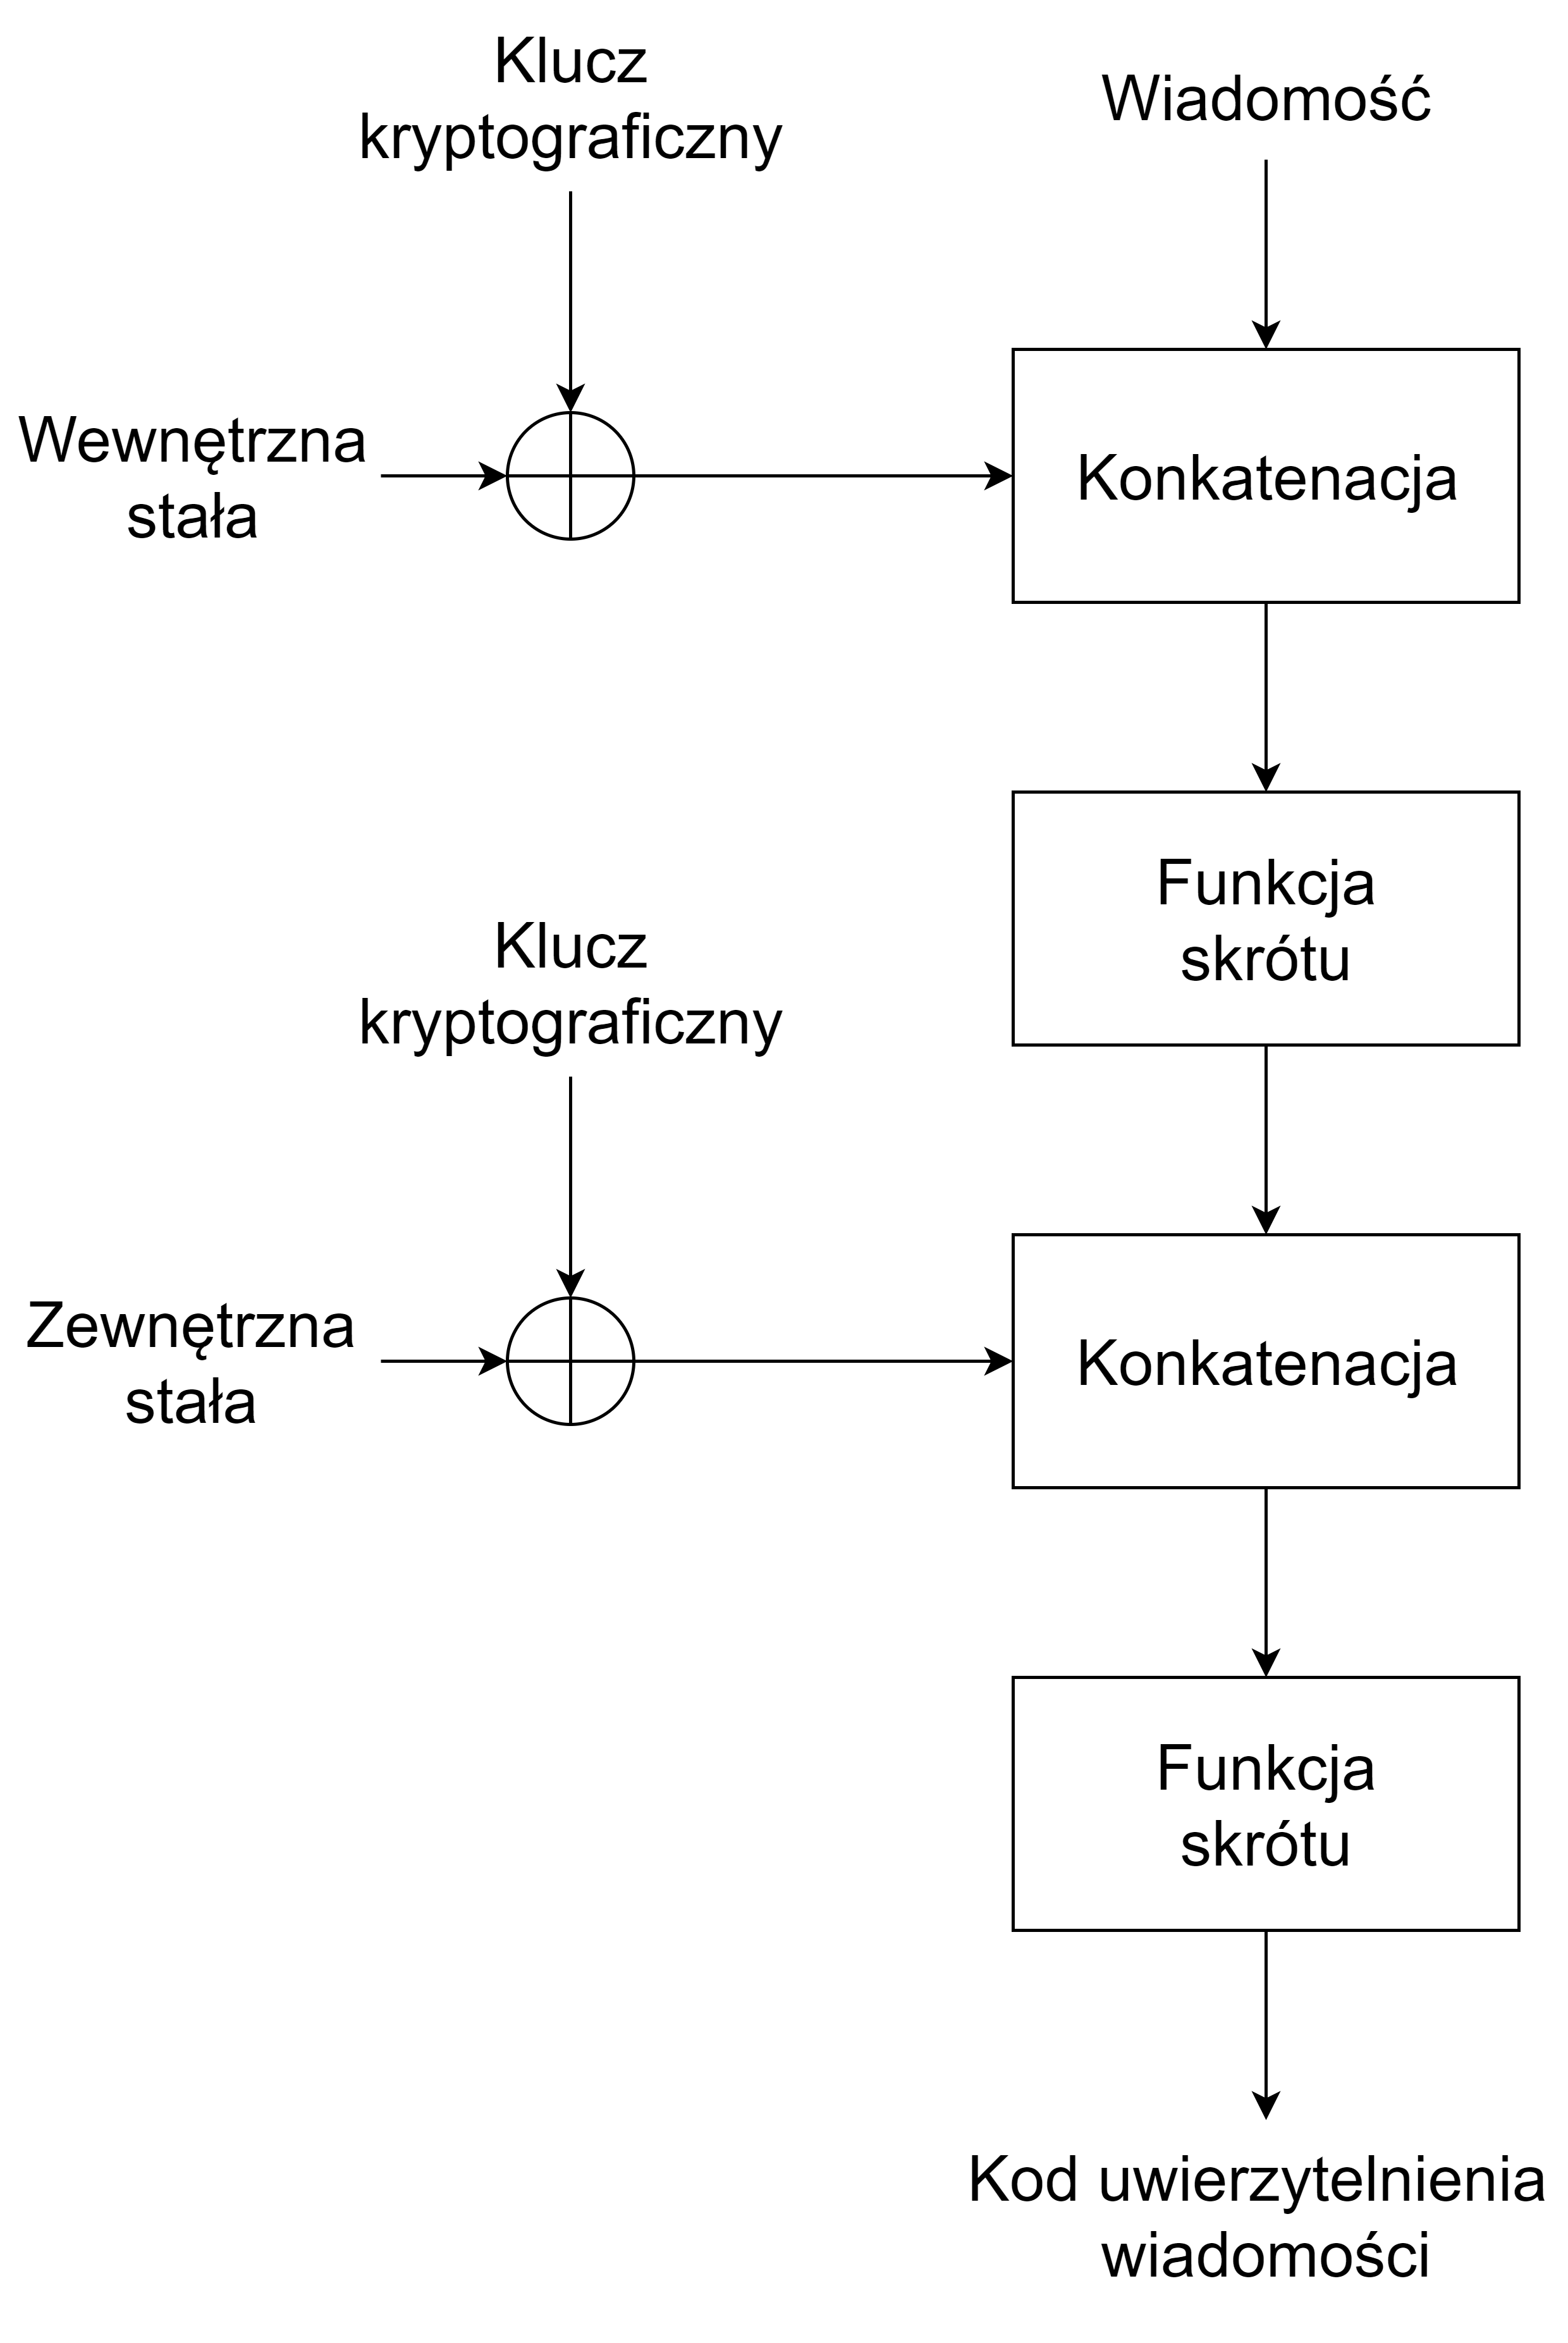
\includegraphics[width=\textwidth, height=\textheight/2, keepaspectratio]{content/images/hmac}
    \caption{Schemat HMAC.}
    \label{hmac-scheme}
\end{figure} 
\noindent
Wartości stałych nie mają tutaj większego znaczenia. Ważne jest jednak aby miały długość równą długości bloku
użytej funkcji skrótu oraz aby były od siebie różne. 
Na etapie konkatenacji wynik działania funkcji XOR jest dostawiany z lewej strony.

\section{Generatory liczb losowych}

\subsection{Pojęcie entropii}
Entropia jest miarą średniej ilości informacji w danej wiadomości. 
Im więcej informacji jest zawartych w wiadomości, tym większa jest jej entropia. \\
Przykładowo dla wiadomości składającej się z samych bitów o wartości 1, entropia wynosi 0 bitów, gdyż wybierając 
losowo jeden z bitów, ze stuprocentowym prawdopodobieństwem otrzymamy bit o wartości 1.
Mając wiadomość o długości 64 bity, w której każdy bit ma losową wartość, entropia wynosi 64 bity.
W przypadku wiadomości o długości 32 znaki, w której mogą pojawić się litery: a, b, c i d,
a prawdopodobieństwo wystąpienia każdej z liter jest równe $25\%$ entropia wynosi 2~bity. \\
Wartość entropii jest liczona za pomocą wzoru:
$$
	H(X) := - \sum_x P(X=x) \log_2 P(X=x)
$$
$P(X=x)$ jest prawdopodobieństwem, że zmienna $X$ przybierze wartość $x$. \\
W zastosowaniach kryptograficznych konieczne jest aby entropia kluczy była wysoka. 
W~przeciwnym razie pojawi się możliwość złamania kluczy metodą siłową.

\subsection{Generatory prawdziwie losowych liczb}
Oczywistym jest fakt, że przy użyciu wyłącznie deterministycznych metod nie jesteśmy w stanie stworzyć
generatorów prawdziwie losowych liczb. Do stworzenia takich generatorów konieczne jest bazowanie na 
zjawiskach fizycznych takich jak procesy termiczne czy procesy kwantowe. \\
Jednym z takich generatorów dostępnych publicznie jest platforma \textit{RANDOM.ORG}, wykorzystująca 
szumy atmosferyczne do generacji liczb prawdziwie losowych.

\subsection{Kryptograficzne generatory liczb pseudolosowych}
Idealnym byłoby używanie generatorów prawdziwie losowych liczb do zastosowań kryptograficznych, takich 
jak na przykład generacja klucza symetrycznego. Często jednak nie mamy dostępu do takich generatorów
lub użycie ich byłoby zbyt kosztowne. Szczęśliwie okazuje się, że do codziennych zastosowań 
wystarczającym jest użycie kryptograficznie bezpiecznych generatorów liczb pseudolosowych. \\ \\
Algorytmami używanymi w kryptografii do generacji liczb pseudolosowych są:
\begin{itemize}
	\item \textit{Yarrow}
	\item \textit{Blum Blum Shub}
	\item \textit{Dual\_EC\_DRBG}
	\item \textit{Mersenne Twister}
\end{itemize}
Warto zaznaczyć, że samodzielna implementacja algorytmów jest wyjątkowo niewskazana. 
Jest to obszar kryptografii, w którym niezwykle łatwo jest popełnić błąd, który
będzie powodował złamanie całego systemu kryptograficznego. \\
W razie potrzeby wygenerowania liczb pseudolosowych zalecane jest użycie interfejsu 
wystawionego przez używany system operacyjny. Na systemach z rodziny \textit{Unix}
interfejsem tym jest \texttt{/dev/urandom}, zaś na systemach \textit{Windows} należy korzystać
z \texttt{CryptGenRandom}.
